% Harus dimuat terlebih dahulu, digunakan agar file PDF memiliki format karakter yang benar.
% Untuk informasi lebih lanjut, lihat https://ctan.org/pkg/cmap.
\RequirePackage{cmap}

% Format dokumen sebagai paper konferensi menggunakan aturan IEEEtran terbaru (v1.8b).
% Untuk informasi lebih lanjut, lihat http://www.michaelshell.org/tex/ieeetran/.
\documentclass[a4paper, conference]{IEEEtran}

% Format encoding font dan input menjadi 8-bit UTF-8.
\usepackage[T1]{fontenc}
\usepackage[utf8]{inputenc}
\usepackage{amsmath}

% Digunakan untuk mengatur margin dokumen.
\usepackage{textcomp}

% Format bahasa menjadi bahasa indonesia dan inggris.
\usepackage[indonesian]{babel}

% Digunakan untuk tujuan demonstrasi.
\usepackage{mwe}

% Digunakan untuk menampilkan font dengan style yang lebih baik.
\usepackage[zerostyle=b,scaled=.75]{newtxtt}

% Digunakan untuk menampilkan tabel dengan style yang lebih baik.
\usepackage{booktabs}
\usepackage[table,xcdraw]{xcolor}
% Digunakan untuk menampilkan gambar pada dokumen.
\usepackage{graphicx}

% Digunakan untuk menampilkan potongan kode.
\usepackage{listings}
\lstset{
  basicstyle=\ttfamily,
  columns=fixed,
  basewidth=.5em,
  xleftmargin=0.5cm,
  captionpos=b
}

\usepackage{amsmath}
\usepackage{amssymb}
\usepackage{physics}
\usepackage{txfonts} % Font times
\usepackage{lipsum}
\usepackage{longtable}
\usepackage{tabularx}
\usepackage{wrapfig}
\usepackage{float}

\usepackage{tikz}
\usepackage{relsize}
\usetikzlibrary{shapes.geometric, arrows, positioning, decorations.pathreplacing, calc}

\tikzset{
  person/.style={
    minimum height=1.6cm, text centered, append after command={
      \pgfextra{
        \draw[thick, fill=green!30] (\tikzlastnode.north) circle (0.4cm);
        \draw[thick] (\tikzlastnode.north) ++(0,-0.4) -- ++(0,-0.8) -- ++(-0.4,-0.4); % Tubuh dan kaki kiri
        \draw[thick] (\tikzlastnode.north) ++(0,-0.4) -- ++(0,-0.8) -- ++(0.4,-0.4);  % Tubuh dan kaki kanan
        \draw[thick] (\tikzlastnode.north) ++(0,-0.4) -- ++(-0.4,-0.4); % Tangan kiri
        \draw[thick] (\tikzlastnode.north) ++(0,-0.4) -- ++(0.4,-0.4);  % Tangan kanan
      }
    }
  },
  motor/.style={
    draw, inner sep=0pt, append after command={
      \pgfextra{
        \draw[thick] (\tikzlastnode.south west) -- (\tikzlastnode.south east)
                    -- ++(0.5,1.5) -- ++(-3,0) -- cycle; % Menggambar trapesium manual
      }
    }
  },
  startstop/.style={ellipse, minimum width=3cm, minimum height=1cm, text centered, draw=black, fill=red!30},
  connector/.style={circle, minimum width=1cm, minimum height=1cm, text centered, draw=black, fill=green!30},
  io/.style={trapezium, trapezium left angle=70, trapezium right angle=110, minimum width=1.5cm, minimum height=1cm, 
                text centered, text width=2.5cm, draw=black, fill=blue!30},
  process/.style={rectangle, minimum width=3cm, minimum height=1cm, text centered, text width=4cm, draw=black, fill=orange!30},
  decision/.style={diamond, aspect=2, minimum width=3cm, minimum height=1cm, inner sep=0, text centered, text width=3cm, draw=black, fill=yellow!30},
  arrow/.style={thick,->,>=stealth, rounded corners},
  layer/.style={rectangle, rounded corners, minimum width=3cm, minimum height=1cm, text centered, align=center, draw=black, fill=blue!30},
  label/.style={align=right, font=\large, anchor=north},
  cbs/.style={rectangle, rounded corners, minimum width=3cm, minimum height=1cm, text centered, align=center, draw=black, fill=blue!20},
  c3k2/.style={rectangle, rounded corners, minimum width=3cm, minimum height=1cm, text centered, align=center, draw=black, fill=yellow!30},
  upsample/.style={rectangle, rounded corners, minimum width=3cm, minimum height=1cm, text centered, draw=black, fill=red!30},
  concat/.style={rectangle, rounded corners, draw=black, fill=blue!50, minimum width=2cm, text centered, minimum height=1cm},
  detect/.style={rectangle, rounded corners, minimum width=1.5cm, minimum height=1cm, text centered, draw=black},
  conv2D/.style={rectangle, rounded corners, minimum width=2cm, minimum height=1cm, text centered, draw=black, fill=magenta!50}
}
% Digunakan agar backticks (`) dapat dirender pada PDF.
% Untuk informasi lebih lanjut, lihat https://tex.stackexchange.com/a/341057/9075.
\usepackage{upquote}

% Digunakan untuk menyeimbangkan bagian akhir dokumen dengan dua kolom.
\usepackage{balance}

% Kapitalisasi caption tabel
\usepackage{caption}
\captionsetup[table]{
    justification=centering, % Memusatkan caption
    labelsep=newline, % Memisahkan label "TABLE 1" dengan judul dengan baris baru
    textfont={sc}, % Membuat teks menjadi kapital
    labelfont={sc} % Membuat teks menjadi kapital
}


% Digunakan untuk menampilkan pustaka.
\usepackage[square,comma,numbers,sort&compress]{natbib}

% Mengubah format ukuran teks pada natbib.
\renewcommand{\bibfont}{\normalfont\footnotesize}

% Jika melebihi 3 penulis dapat dilakukan linebreakend 
\makeatletter
\newcommand{\linebreakand}{%
  \end{@IEEEauthorhalign}
  \hfill\mbox{}\par
  \mbox{}\hfill\begin{@IEEEauthorhalign}
}
\makeatother

% Menambah nama penulis ketika menggunakan perintah \citet.
% Untuk informasi lebih lanjut, lihat https://tex.stackexchange.com/a/76075/9075.
\usepackage{etoolbox}
\makeatletter
\patchcmd{\NAT@test}{\else \NAT@nm}{\else \NAT@hyper@{\NAT@nm}}{}{}
\makeatother

% Digunakan untuk melakukan linewrap pada pustaka dengan url yang panjang
% jika terdapat hyphens
\usepackage[hyphens]{url}

% Digunakan untuk menambah hyperlink pada referensi.
\usepackage{hyperref}

% Menonaktifkan warna dan bookmark pada hyperref.
\hypersetup{hidelinks,
  colorlinks=true,
  allcolors=black,
  pdfstartview=Fit,
  breaklinks=true
}

% Digunakan untuk membenarkan hyperref pada gambar.
\usepackage[all]{hypcap}

% Digunakan untuk menampilkan beberapa gambar
%\usepackage[caption=false,font=footnotesize]{subfig}
\usepackage{multirow}
\usepackage{longtable}
\usepackage{graphicx}
\usepackage{subcaption}
\usepackage{stfloats}
\usepackage{float}
% nama
\newcommand{\name}{Aldi Fahmi Sihotang}
\newcommand{\authorname}{Sihotang, Aldi Fahmi}
\newcommand{\nickname}{Aldi}
\newcommand{\advisor}{Dr. Eko Mulyanto Yuniarno, S.T., M.T.}
\newcommand{\coadvisor}{Dr. Supeno Mardi Susiki Nugroho,S.T.,M.T.}

% identitas
\newcommand{\nrp}{0721 18 4000 0039}
\newcommand{\advisornip}{19680601 199512 1 009}
\newcommand{\coadvisornip}{19700313199512 1 001}
\newcommand{\email}{07211840000039@student.its.ac.id}
\newcommand{\advisoremail}{ekomulyanto@ee.its.ac.id}
\newcommand{\coadvisoremail}{mardi@its.ac.id}

% judul
\newcommand{\tatitle}{PENGEMBANGAN KURSI RODA OTONOM UNTUK MENGIKUTI MANUSIA BERBASIS \emph{YOLOv11}}
\newcommand{\engtatitle}{YOLOv11-BASED AUTONOMOUS WHEELCHAIR DEVELOPMENT FOR FOLLOWING HUMAN}
% tempat
\newcommand{\place}{Surabaya}   

% jurusan
\newcommand{\studyprogram}{Teknik Komputer}
\newcommand{\engstudyprogram}{Computer Engineering}

% fakultas
\newcommand{\faculty}{Teknologi Elektro dan Informatika Cerdas}
\newcommand{\engfaculty}{Intelligence Electrical and Informatics Technology}

% singkatan fakultas
\newcommand{\facultyshort}{FTEIC}
\newcommand{\engfacultyshort}{ELECTICS}

% departemen
\newcommand{\department}{Teknik Komputer}
\newcommand{\engdepartment}{Computer Engineering}

% Tambahkan format tanda hubung yang benar di sini
\hyphenation{
  ro-ket
  me-ngem-bang-kan
  per-hi-tu-ngan
}


\begin{document}

% Ubah kalimat berikut sesuai dengan judul penelitian.
\title{\tatitle{}}

% Ubah kalimat-kalimat berikut sesuai dengan nama, institusi, alamat dan kontak penulis.
\author{
  \IEEEauthorblockN{\advisor{}}
  \IEEEauthorblockA{\textit{Departemen \studyprogram{}}\\
    \textit{Institut Teknologi Sepuluh Nopember}\\
    Surabaya, Indonesia 60111\\
    \advisoremail{}}

  \and
  \IEEEauthorblockN{\coadvisor{}}
  \IEEEauthorblockA{\textit{Departemen \studyprogram{}}\\
    \textit{Institut Teknologi Sepuluh Nopember}\\
    Surabaya, Indonesia 60111\\
    \coadvisoremail{}}

  \and
  \IEEEauthorblockN{\name{}}
  \IEEEauthorblockA{\textit{Departemen \studyprogram{}}\\
    \textit{Institut Teknologi Sepuluh Nopember}\\
    Surabaya, Indonesia 60111\\
    \email{}}
}

% Digunakan untuk menampilkan judul dan deskripsi penulis.
\maketitle
% Mengubah keterangan `Abstract` ke bahasa indonesia.
% Hapus bagian ini untuk mengembalikan ke format awal.
\renewcommand\abstractname{Abstrak}

\begin{abstract}

  % Ubah paragraf berikut sesuai dengan abstrak dari penelitian.
  Penelitian ini bertujuan untuk mengembangkan sistem kendali kursi roda otonom yang dapat mengikuti pergerakan manusia secara real-time. Sistem ini mengintegrasikan algoritma deteksi objek \emph{YOLOv11} dan pelacakan gerakan tubuh menggunakan \emph{MediaPipe Pose}, dengan memanfaatkan sudut pandang optimal sebagai dasar pengambilan data visual. Kamera ditempatkan pada kacamata pengguna untuk mendapatkan sudut pandang yang optimal dalam mendeteksi dan melacak pergerakan pengguna. Sistem ini dirancang agar dapat beroperasi secara nirkabel menggunakan modul \emph{ESP32}, memberikan fleksibilitas dan efisiensi dalam mengendalikan pergerakan kursi roda. Pengujian dilakukan dalam lingkungan terkendali untuk memastikan keakuratan dan kecepatan deteksi serta pelacakan gerakan pengguna. Hasil penelitian menunjukkan bahwa sistem dapat mengikuti pergerakan pengguna dengan akurat dan responsif, memberikan kontribusi signifikan terhadap pengembangan teknologi mobilitas kesehatan yang lebih cerdas dan mandiri.

\end{abstract}

% Mengubah keterangan `Index terms` ke bahasa indonesia.
% Hapus bagian ini untuk mengembalikan ke format awal.
\renewcommand\IEEEkeywordsname{Kata kunci}

\begin{IEEEkeywords}

  % Ubah kata-kata berikut sesuai dengan kata kunci dari penelitian.
  Kursi Roda Otonom, YOLOv11, MediaPipe Pose, Sudut Pandang Optimal, Deteksi Gerakan, Kendali Nirkabel, Mobilitas Kesehatan

\end{IEEEkeywords}


% Ubah bagian berikut sesuai dengan konten-konten yang akan dimasukkan pada dokumen
% Ubah judul dan label berikut sesuai dengan yang diinginkan.
\section{Pendahuluan}
\label{sec:pendahuluan}

Teknologi \emph{Internet of Things (IoT)} dan \emph{deep learning} semakin banyak diadopsi dalam pengembangan sistem kendali otonom, khususnya untuk aplikasi kesehatan dan mobilitas. Kursi roda otonom merupakan salah satu solusi yang dapat meningkatkan kualitas hidup penyandang disabilitas dengan memberikan kemandirian dalam bergerak. Salah satu teknologi utama yang dapat mendukung pengembangan kursi roda otonom adalah modul \emph{ESP32}. Berdasarkan penelitian yang dilakukan oleh \emph{Ekatama} (2024), \emph{ESP32} mampu mengendalikan perangkat secara nirkabel dengan memanfaatkan konektivitas \emph{Wi-Fi} dan \emph{Bluetooth}, memberikan fleksibilitas yang lebih besar dalam mengontrol kursi roda. Penggunaan modul ini memungkinkan pengguna untuk mengontrol kursi roda secara efektif tanpa perlu mengandalkan kontrol manual yang terbatas \cite{ekatama2024perancangan}.

Selain aspek kendali nirkabel, sistem otonom yang mengikuti pergerakan pengguna membutuhkan teknologi yang mampu mendeteksi gerakan tubuh secara real-time. Penelitian oleh \emph{Wijaya et al.} (2022) telah menunjukkan keandalan algoritma \emph{YOLO V3} dalam mendeteksi objek secara cepat dan akurat, yang dapat digunakan untuk melacak pergerakan manusia. Namun, dalam penelitian ini, algoritma \emph{YOLOv11}, versi terbaru dari \emph{YOLO}, diintegrasikan dengan \emph{MediaPipe Pose}, sebuah framework yang dapat mendeteksi dan melacak posisi tubuh manusia. Kombinasi kedua teknologi ini memungkinkan sistem untuk secara akurat mengikuti gerakan pengguna berdasarkan sudut pandang optimal yang diperoleh dari kamera yang dipasang pada kacamata pengguna. Dengan pendekatan ini, kursi roda dapat mengikuti pergerakan pengguna secara alami, mendukung otonomi yang lebih tinggi \cite{wijaya2022deteksi}.

Sistem kursi roda otonom yang dikembangkan dalam penelitian ini memanfaatkan modul \emph{ESP32} sebagai perangkat keras utama yang mengontrol keseluruhan sistem secara nirkabel. Dalam penelitian yang dilakukan oleh \emph{Narwaria et al.} (2024), \emph{ESP32-CAM} telah terbukti mampu menangkap dan mengolah data visual dengan efisiensi tinggi, yang dapat diterapkan untuk berbagai aplikasi berbasis \emph{IoT}. Sistem yang dikembangkan tidak hanya dirancang untuk mendeteksi objek, tetapi lebih berfokus pada pelacakan gerakan tubuh pengguna melalui teknologi \emph{MediaPipe Pose}. Dengan integrasi ini, sistem dapat memastikan bahwa pergerakan kursi roda tetap sejalan dengan pergerakan pengguna tanpa memerlukan input manual tambahan \cite{10696374}.

Dengan latar belakang ini, proyek ini bertujuan untuk mengembangkan sistem kursi roda otonom yang dapat mengikuti pergerakan pengguna secara real-time, dengan rancangan dan implementasi sistem kendali kursi roda yang dapat mengikuti pergerakan pengguna dengan memanfaatkan sudut pandang optimal dari kamera yang ditempatkan pada kacamata.

% Ubah judul dan label berikut sesuai dengan yang diinginkan.
\section{Tinjauan Pustaka}
\label{sec:tinjauanpustaka}

\subsection{Object Detection}
\label{subsec:detection}

\emph{Object detection} atau deteksi objek adalah teknologi inti dalam banyak aplikasi modern seperti sistem pengawasan, pengenalan wajah, dan kendaraan otonom. Teknologi ini digunakan untuk mendeteksi dan mengklasifikasikan berbagai objek dalam gambar atau video. Dalam konteks penelitian ini, \emph{object detection} berperan penting untuk mendeteksi keberadaan manusia sehingga kursi roda otonom dapat mengikuti gerakan pengguna secara real-time. Perkembangan pesat dalam \emph{deep learning}, terutama dengan penggunaan \emph{Convolutional Neural Network} (CNN), telah mengoptimalkan kemampuan \emph{object detection}. \emph{CNN}, dengan berbagai lapisannya seperti lapisan konvolusi, aktivasi, \emph{pooling}, dan \emph{fully connected}, menjadi fondasi dari banyak metode deteksi objek saat ini, termasuk \emph{YOLO} (You Only Look Once).

\emph{YOLO}, salah satu metode deteksi objek paling populer, mampu melakukan deteksi dengan kecepatan tinggi dan akurasi yang baik, menjadikannya sangat cocok untuk aplikasi \emph{real-time} seperti kursi roda otonom. \emph{YOLOv11}, versi terbaru dari keluarga \emph{YOLO}, menawarkan peningkatan signifikan dalam kecepatan dan akurasi, serta tambahan fitur seperti \emph{YOLO pose} untuk deteksi pose manusia. Selain itu, metode pelacakan objek seperti \emph{DeepSORT} yang menggunakan \emph{Kalman Filter} dan \emph{Hungarian Algorithm}, serta teknologi lainnya seperti \emph{MediaPipe Pose}, semakin memperkuat kemampuan sistem kursi roda otonom dalam melacak dan mengikuti gerakan manusia dengan presisi tinggi.

\subsection{Convolutional Neural Network (CNN)}
\label{subsec:cnn}

\emph{Convolutional Neural Network} (CNN) adalah jenis jaringan saraf tiruan yang dirancang khusus untuk pengolahan data yang memiliki struktur grid, seperti gambar. CNN terdiri dari serangkaian lapisan yang bekerja sama untuk mengekstraksi dan menganalisis fitur dari data input, membuatnya sangat efektif dalam tugas-tugas seperti klasifikasi gambar, segmentasi, dan deteksi objek.

\subsubsection{Lapisan Konvolusi (\emph{Convolutional Layer})}
\label{subsubsec:Convolutional Layer}

Lapisan konvolusi adalah fondasi dari CNN yang bertugas mengekstraksi fitur-fitur penting dari input gambar. Dengan menerapkan filter yang dipelajari selama pelatihan, lapisan ini mampu mengenali elemen-elemen dasar seperti tepi, tekstur, dan pola dalam gambar. Setiap filter dalam lapisan konvolusi bertanggung jawab untuk mendeteksi fitur tertentu, dan hasilnya disusun dalam peta fitur (\emph{feature map}) yang memberikan representasi visual dari elemen-elemen yang terdeteksi. Formula untuk operasi konvolusi dapat dituliskan sebagai berikut:

\begin{equation}
  (f * g)(t) = \int_{-\infty}^{\infty} f(\tau)g(t - \tau) \, d\tau
\end{equation}

\subsubsection{Lapisan Aktivasi (\emph{Activation Layer})}
\label{subsubsec:Activation Layer}

Lapisan aktivasi adalah komponen yang menambahkan non-linearitas ke dalam jaringan, yang memungkinkan model untuk mempelajari hubungan yang lebih kompleks. Fungsi aktivasi seperti \emph{ReLU} (\emph{Rectified Linear Unit}) digunakan untuk mengaktifkan neuron hanya jika outputnya positif, sehingga mengurangi kompleksitas komputasi dan mempercepat proses pelatihan. Non-linearitas ini sangat penting untuk mengatasi masalah yang melibatkan data dengan struktur yang rumit, seperti deteksi objek dalam gambar.

\subsubsection{Lapisan \emph{Pooling} (\emph{Pooling Layer})}
\label{subsubsec:Pooling Layer}

Lapisan \emph{pooling} digunakan untuk mengurangi dimensi peta fitur sambil mempertahankan informasi yang paling relevan. Metode \emph{pooling} seperti \emph{max pooling} mengambil nilai maksimum dalam setiap area \emph{pooling}, yang membantu jaringan menjadi lebih tahan terhadap variasi kecil dalam input, seperti perubahan skala atau rotasi objek. Dengan mereduksi jumlah data yang harus diproses, \emph{pooling} juga membantu mengurangi risiko \emph{overfitting} dan mempercepat pelatihan. Operasi \emph{max pooling} dapat direpresentasikan sebagai:

\begin{equation}
  P(x, y) = \max_{i,j \in \mathrm{PoolRegion}} I(x+i, y+j)
\end{equation}

\subsubsection{Lapisan \emph{Fully Connected} (\emph{Fully Connected Layer})}
\label{subsubsec:Fully Connected Layer}

Lapisan \emph{fully connected} adalah lapisan terakhir dalam CNN yang menghubungkan setiap neuron di lapisan sebelumnya ke setiap neuron di lapisan ini. Lapisan ini berfungsi untuk menggabungkan semua fitur yang telah diekstraksi oleh lapisan konvolusi dan \emph{pooling}, dan menghasilkan output akhir, seperti prediksi kelas objek. Lapisan \emph{fully connected} memegang peran penting dalam memproses informasi yang dihasilkan dari lapisan-lapisan sebelumnya untuk membuat keputusan akhir tentang klasifikasi atau deteksi. Rumus dasar untuk operasi \emph{fully connected} dapat dituliskan sebagai:

\begin{equation}
  y = f\left(\sum_{i=1}^{n} w_i x_i + b\right)
\end{equation}

Dimana \( w_i \) adalah bobot, \( x_i \) adalah input, \( b \) adalah bias, dan \( f \) adalah fungsi aktivasi.

\subsection{Pose Estimation}
\label{subsec:Pose Estimation}

\emph{Pose estimation} adalah teknik untuk mengidentifikasi dan melacak posisi tubuh manusia dalam gambar atau video. Teknik ini biasanya melibatkan deteksi titik-titik kunci (\emph{keypoints}) pada tubuh, seperti sendi atau ujung-ujung anggota tubuh, yang digunakan untuk memodelkan postur atau gerakan individu. \emph{Pose estimation} sangat penting dalam berbagai aplikasi, seperti analisis olahraga, animasi, dan interaksi manusia-mesin.

Dalam penelitian ini, \emph{pose estimation} digunakan untuk memastikan gerakan pengguna dapat diikuti dengan akurasi tinggi. Dengan memanfaatkan \emph{pose estimation}, sistem dapat memahami arah dan intensitas gerakan pengguna, yang memungkinkan kursi roda untuk merespons secara tepat dan efisien.

\subsection{YOLO (\emph{You Only Look Once})}
\label{subsec:YOLO}

\emph{YOLO}, yang dikembangkan oleh Joseph Redmon, memperkenalkan pendekatan \emph{End-to-End} untuk deteksi objek dalam \emph{Real-Time}. Nama \emph{YOLO}, singkatan dari \emph{"You Only Look Once"} (Anda Hanya Melihat Sekali), mencerminkan kemampuan model ini dalam menyelesaikan tugas deteksi hanya dengan satu kali pemrosesan jaringan. Hal ini berbeda dengan pendekatan sebelumnya, yang menggunakan teknik \emph{sliding window} dan memerlukan pengklasifikasi yang harus dijalankan berkali-kali pada setiap gambar, atau metode lain yang memecah tugas menjadi dua langkah terpisah: pertama, mengidentifikasi daerah yang mungkin mengandung objek (\emph{region proposals}), dan kedua, menjalankan pengklasifikasi pada daerah yang telah diidentifikasi tersebut. Selain itu, \emph{YOLO} memanfaatkan \emph{output} yang lebih sederhana dengan hanya menggunakan regresi untuk memprediksi hasil deteksi, berlawanan dengan metode seperti \emph{Fast R-CNN} yang memisahkan tugas menjadi dua \emph{output} terpisah: probabilitas klasifikasi dan regresi untuk koordinat \emph{bounding box}.

\subsubsection{YOLOv8}
\label{subsubsec:YOLOv8}

\emph{YOLOv8} adalah salah satu model deteksi objek yang sangat efisien, menggabungkan kecepatan tinggi dengan akurasi yang relatif tinggi. Arsitektur ini terdiri dari beberapa lapisan utama: \emph{Backbone}, \emph{Neck}, dan \emph{Head}. \emph{Backbone} bertugas untuk mengekstraksi fitur-fitur dasar dari gambar input. Kemudian, \emph{Neck} menggabungkan informasi dari berbagai lapisan untuk menghasilkan representasi fitur yang lebih kaya, yang kemudian diproses oleh \emph{Head} untuk menghasilkan prediksi \emph{bounding box}, label kelas, dan skor \emph{confidence}.

\begin{figure}[H] 
  \centering 
  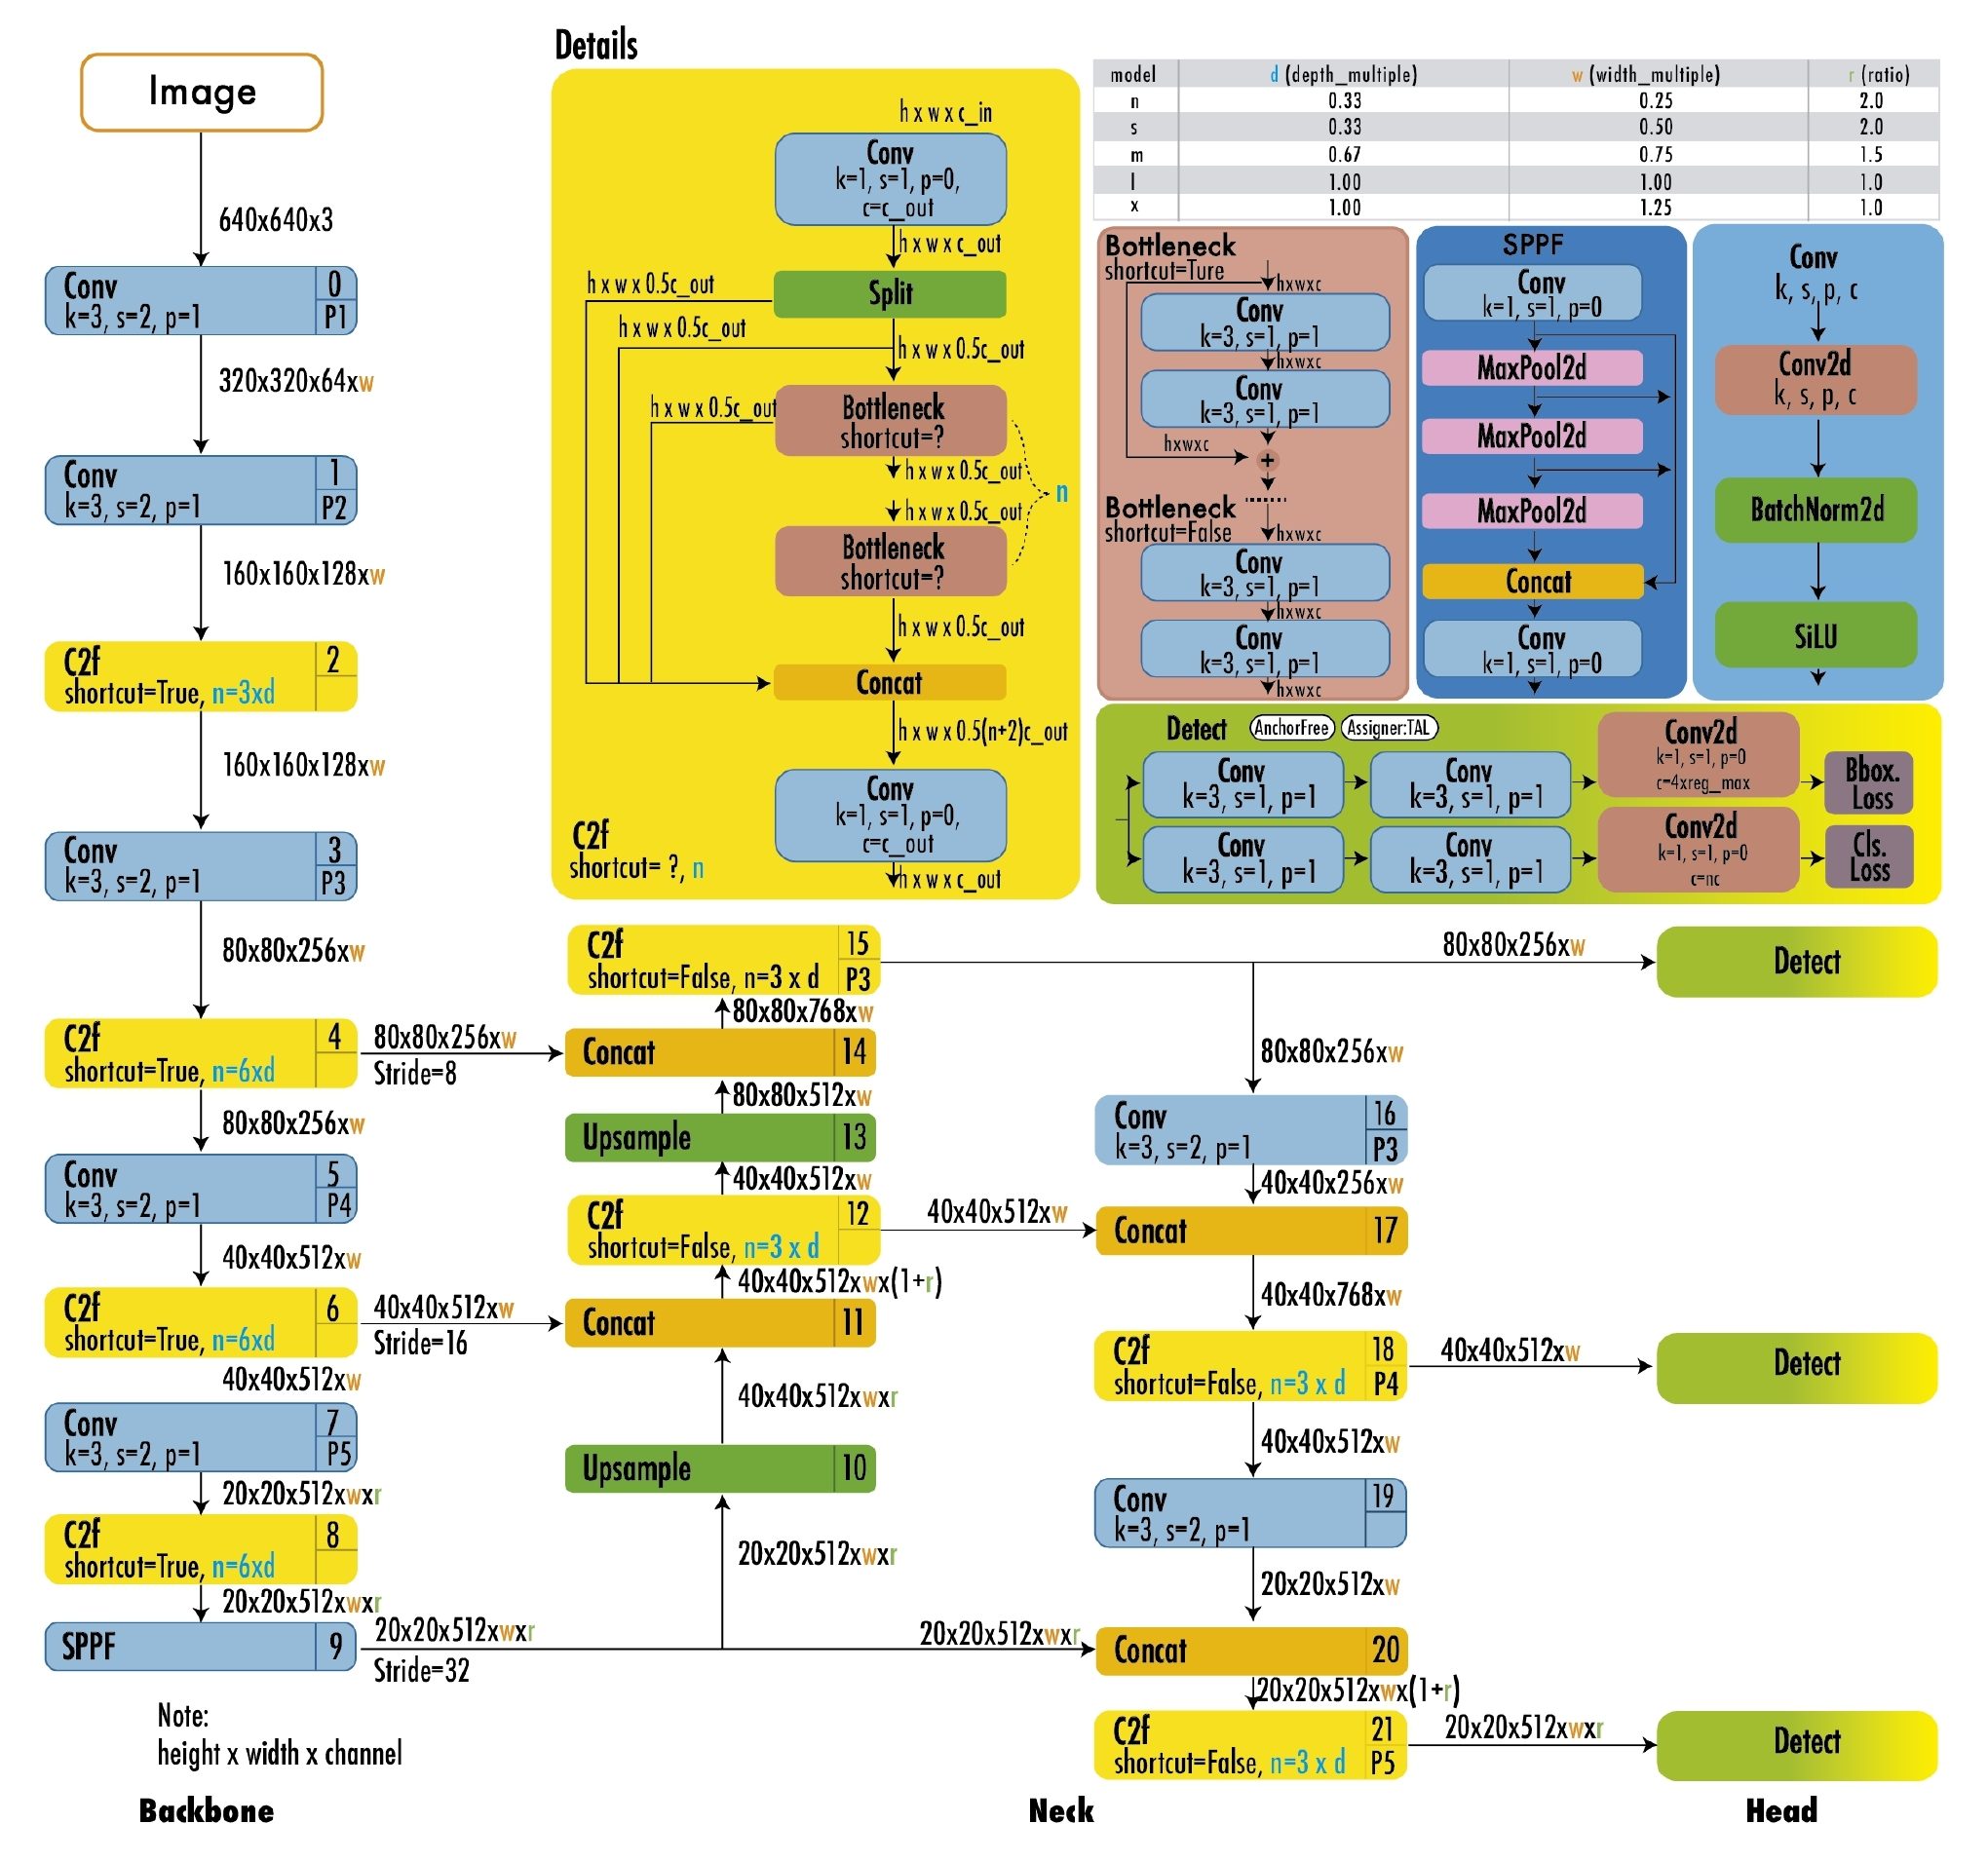
\includegraphics[scale=0.5]{gambar/YoloV8Architecture.jpg} 
  \caption{Arsitektur YOLOv8.} 
  \label{fig:ArsitekturYOLOv8} 
\end{figure}

Gambar menunjukkan arsitektur lengkap \emph{YOLOv8}, dimulai dari input gambar dengan resolusi 640x640x3, yang diproses melalui serangkaian lapisan konvolusi dalam \emph{Backbone} untuk mengekstraksi fitur penting. Kemudian, fitur-fitur ini diteruskan melalui \emph{Neck} yang menggabungkan dan mengolah informasi dari berbagai level resolusi, menghasilkan representasi multi-skala yang kaya. Akhirnya, \emph{Head} bertanggung jawab untuk melakukan prediksi akhir, seperti \emph{bounding boxes}, label kelas, dan \emph{confidence score}.

\emph{YOLOv8} memprediksi \emph{bounding box} menggunakan kombinasi antara koordinat pusat \((bx, by)\), dimensi \emph{bounding box} \((bw, bh)\), dan skor \emph{confidence} \(p_c\). Formula untuk menghitung koordinat \emph{bounding box} berdasarkan \emph{output} jaringan adalah:

\begin{equation}
  \begin{array}{c}
  bx = \sigma(t_x) + c_x\\
  bw = p_w e^{t_w}\\
  by = \sigma(t_y) + c_y\\ 
  bh = p_h e^{t_h}
  \end{array}
\end{equation}

Di mana \(t_x, t_y, t_w, t_h\) adalah \emph{output} dari model \emph{neural network}, \(\sigma\) adalah fungsi sigmoid, \(c_x, c_y\) adalah koordinat \emph{grid cell}, dan \(p_w, p_h\) adalah skala \emph{anchor box}.

Fungsi \emph{loss} dalam \emph{YOLOv8} terdiri dari beberapa komponen utama yang mengukur perbedaan antara prediksi model dan \emph{ground truth}, serta menyeimbangkan pentingnya prediksi koordinat, \emph{confidence score}, dan klasifikasi objek. Rumus fungsi \emph{loss}-nya adalah:

\begin{equation}
  \begin{array}{c}
  \mathbf{Loss} = \lambda_{\mathrm{coord}} \sum_{i=0}^{S^2} \sum_{j=0}^{B} \mathbb{1}_{ij}^{\mathrm{obj}} \left[ (bx_i - \hat{bx}_i)^2 + (by_i - \hat{by}_i)^2 \right] \\[10pt]
  + \lambda_{\mathrm{coord}} \sum_{i=0}^{S^2} \sum_{j=0}^{B} \mathbb{1}_{ij}^{\mathrm{obj}} \left[ (\sqrt{bw_i} - \sqrt{\hat{bw}_i})^2 + (\sqrt{bh_i} - \sqrt{\hat{bh}_i})^2 \right] \\[10pt]
  + \sum_{i=0}^{S^2} \sum_{j=0}^{B} \mathbb{1}_{ij}^{\mathrm{obj}} (C_i - \hat{C}_i)^2 + \lambda_{\mathrm{noobj}} \sum_{i=0}^{S^2} \sum_{j=0}^{B} \mathbb{1}_{ij}^{\mathrm{noobj}} (C_i - \hat{C}_i)^2 \\[10pt]
  + \sum_{i=0}^{S^2} \mathbb{1}_{i}^{\mathrm{obj}} \sum_{c \in \mathrm{classes}} (p_i(c) - \hat{p}_i(c))^2
  \end{array}
\end{equation}

Pada persamaan ini, \(S\) adalah ukuran grid, \(B\) adalah jumlah \emph{bounding boxes} per \emph{grid cell}, \(\mathbb{1}_{ij}^{\mathrm{obj}}\) adalah indikator bahwa \emph{bounding box} j di \emph{cell} i memprediksi objek, dan \(\lambda_{\mathrm{coord}}\) dan \(\lambda_{\mathrm{noobj}}\) adalah hyperparameter yang mengontrol pentingnya masing-masing \emph{loss}.

\subsubsection{YOLOv8 Pose}
\label{subsubsec: YOLOv8 Pose}

\emph{YOLOv8 Pose} adalah varian dari \emph{YOLOv8} yang dirancang khusus untuk tugas \emph{pose estimation}. Dengan menggunakan pendekatan yang menggabungkan kecepatan \emph{YOLO} dengan kemampuan deteksi pose yang presisi, \emph{YOLOv8 Pose} mampu mendeteksi titik-titik kunci pada tubuh manusia secara \emph{real-time}. Setiap \emph{bounding box} tidak hanya mengandung informasi tentang lokasi dan ukuran objek, tetapi juga koordinat titik-titik kunci yang terkait dengan pose manusia (misalnya, bahu, siku, lutut, dan sebagainya).

\subsubsection{YOLOv10}
\label{subsubsec:YOLOv10}

\emph{YOLOv10} merupakan pengembangan lebih lanjut dari \emph{YOLOv8}, dengan beberapa perbaikan dalam efisiensi dan akurasi deteksi objek. Seperti \emph{YOLOv8}, arsitektur \emph{YOLOv10} terdiri dari \emph{Backbone}, \emph{Neck}, dan \emph{Head}, namun dengan penambahan beberapa modul baru seperti \emph{Path Aggregation Network} (\emph{PSA}) dan \emph{Improved Convolutional Block} (\emph{C2fCIB}).

Arsitektur \emph{YOLOv10} dikembangkan dengan memperkenalkan beberapa peningkatan kunci dari dasar-dasar \emph{YOLOv8}. \emph{Backbone YOLOv10} tetap berfungsi sebagai ekstraktor fitur utama, namun ditingkatkan dengan modul \emph{SCD} (\emph{Squeeze-and-Excitation Convolutional Downsample}) dan \emph{C2fCIB}, yang memungkinkan propagasi informasi yang lebih efisien dan reduksi redundansi. Modul \emph{PSA} (\emph{Path Aggregation Network}) yang baru ditambahkan dalam \emph{Neck} membantu menggabungkan informasi dari berbagai jalur dalam jaringan, memperkaya representasi fitur untuk deteksi multi-skala.

\subsubsection{YOLOv11}
\label{subsubsec:YOLOv11}

YOLO11 adalah terobosan terbaru dalam seri detektor objek real-time dari Ultralytics. Meneruskan kemajuan dari pendahulunya, YOLO11 menghadirkan peningkatan signifikan pada arsitekturnya, menjadikannya solusi yang kuat dan adaptif untuk berbagai aplikasi \emph{computer vision}. \emph{Ultralytics} memperkenalkan berbagai peningkatan dalam deteksi objek dan arsitektur pembelajaran mendalam. Arsitektur \emph{backbone} dan \emph{neck} yang ditingkatkan memperbaiki ekstraksi fitur, memungkinkan deteksi objek yang lebih akurat dan penanganan tugas yang lebih kompleks. 

Efisiensi dan kecepatan juga dipertajam melalui arsitektur yang disempurnakan dan \emph{pipeline} pelatihan yang lebih optimal, sehingga pemrosesan menjadi lebih cepat tanpa mengorbankan akurasi dan performa. \emph{YOLO11} mendukung implementasi di berbagai platform, mulai dari perangkat \emph{edge}, platform \emph{cloud}, hingga sistem dengan \emph{GPU NVIDIA}, membuatnya fleksibel untuk digunakan di berbagai lingkungan. Selain itu, \emph{YOLO11} mendukung beragam tugas, termasuk deteksi objek, segmentasi \emph{instance}, klasifikasi gambar, estimasi \emph{pose}, dan deteksi objek terorientasi (\emph{OBB}). Salah satu pembaruan utama dalam arsitektur \emph{YOLO11} adalah pengenalan modul \emph{C3K2} yang menggantikan modul \emph{C2F} pada \emph{YOLOv8}, serta penambahan modul \emph{C2PSA} setelah modul \emph{SPPF} untuk meningkatkan kapabilitas deteksi lebih lanjut.

\begin{figure}[H]
  \centering
  \resizebox{1\linewidth}{!}{
    \begin{tikzpicture}[node distance=1.5cm]
% Backbone Nodes
\node (input) [label] {Input};
\node (cbs0) [cbs, above of=input, yshift=1cm] {CBS\\k=3, s=2, p=1};
\node (cbs1) [cbs, above of=cbs0] {CBS\\k=3, s=2, p=1};
\node (c3k2_1) [c3k2, above of=cbs1] {C3K2\\C3k=Fa  lse};
\node (cbs2) [cbs, above of=c3k2_1] {CBS\\k=3, s=2, p=1};
\node (c3k2_2) [c3k2, above of=cbs2] {C3K2\\C3k=False};
\node (cbs3) [cbs, above of=c3k2_2] {CBS\\k=3, s=2, p=1};
\node (c3k2_3) [c3k2, above of=cbs3] {C3K2\\C3k=True};
\node (cbs4) [cbs, above of=c3k2_3] {CBS\\k=3, s=2, p=1};
\node (c3k2_4) [c3k2, above of=cbs4] {C3K2\\C3k=True};
\node (sppf) [layer, above of=c3k2_4, fill=green!20, align=center] {SPPF};
\node (c2psa) [layer, above of=sppf, fill=green!20, align=center] {C2PSA};

% Neck Nodes
\node (up1) [upsample, right of=sppf, xshift=2.25cm, minimum width=2cm] {Upsample};
\node (cc1) [concat, right of=up1, xshift=.5cm] {Concat};
\node (c3k2_5) [c3k2, right of=cc1, xshift=1cm] {C3K2\\C3k=False};

\node (up2) [upsample, below of=c3k2_5, minimum width=2cm] {Upsample};
\node (cc2) [concat, right of=up2, xshift=.5cm] {Concat};
\node (c3k2_6) [c3k2, right of=cc2, xshift=1cm] {C3K2\\C3k=False};

\node (cbs5) [cbs, above of=c3k2_6] {CBS\\k=3, s=2, p=1};
\node (cc3) [concat, right of=cbs5, xshift=1cm] {Concat};
\node (c3k2_7) [c3k2, right of=cc3, xshift=1cm] {C3K2\\C3k=False};

\node (cbs6) [cbs, above of=c3k2_7] {CBS\\k=3, s=2, p=1};
\node (cc4) [concat, right of=cbs6, xshift=1cm] {Concat};
\node (c3k2_8) [c3k2, right of=cc4, xshift=1cm] {C3K2\\C3k=True};

% Head Nodes
\node (detect1) [detect,  right of=c3k2_8, xshift=2cm] {Detect};
\node (detect2) [detect, below of=detect1] {Detect};
\node (detect3) [detect, below of=detect2] {Detect};

% SPPF Diagram
\node (cbs7) [cbs, right of=c3k2_3, xshift=4.75cm] {CBS \\ $k=1, s=1, p=1$};
\node (maxpool1) [layer, fill=red!30, below of=cbs7] {Maxpool};
\node (maxpool2) [layer, fill=red!30, below of=maxpool1] {Maxpool};
\node (maxpool3) [layer, fill=red!30, below of=maxpool2] {Maxpool};
\node (cc5) [concat, fill=blue!50, below of=maxpool3] {Concat};
\node (cbs8) [cbs, below of=cc5] {CBS \\ $k=1, s=1, p=1$};

% C2PSA Diagram
\node (cbs9) [cbs, right of=cbs7, xshift=4.75cm, yshift=.5cm] {CBS \\ $k=1, s=1, p=0$};
\node (split1) [layer, fill=cyan!30, below of=cbs9] {Split};
\node (PSA1) [layer, fill=purple!20, below of=split1] {PSABlock};
\node (dots) [label, below of=PSA1] {...};
\node (PSA2) [layer, fill=purple!20, below of=dots] {PSABlock};
\node (cc6) [concat, fill=blue!50, below of=PSA2] {Concat};
\node (cbs10) [cbs, below of=cc6] {CBS \\ $k=1, s=1, p=0$};

\node (attention) [layer, fill=cyan!30, right of=maxpool2, xshift=9.75cm] {Attention};
\node (cbs11) [cbs, below of=attention, yshift=-1.5cm] {CBS \\ $k=1, s=1, p=0$};
\node (cbs12) [cbs, below of=cbs11] {CBS \\ $k=1, s=1, p=0$};
\node (n1) [label, below of=cbs12] { };
\node (ffn) [label, above of=cbs11, xshift=-1cm, yshift=-.7cm] {FFN};
\node (h1) [label, above of=attention] { };

% CBS
\node (conv2d) [conv2D, right of=cbs9, minimum width=2cm, xshift=7.5cm] {Conv2D};
\node (bN) [layer, right of=conv2d, fill=orange!50, minimum width=1.5cm, xshift=.75cm] {BN};
\node (siLU) [layer, right of=bN, fill=yellow!50, minimum width=2cm, xshift=.75cm] {SiLU};

% Detection
\node (cbs22) [cbs, right of=PSA2, xshift=8cm] {CBS\\k=3, s=1, p=1};
\node (cbs21) [cbs, above of=cbs22] {CBS\\k=3, s=1, p=1};
\node (conv2d_1) [conv2D, below of=cbs22] {Conv2D};
\node (bbox) [layer, below of=conv2d_1, fill=red!50, minimum width=2cm,] {Bbox\\Loss};
\node (h2) [label, above of=cbs21] { };

\node (cbs31) [cbs, right of=cbs21, xshift=2cm] {CBS\\k=3, s=1, p=1};
\node (cbs32) [cbs, below of=cbs31] {CBS\\k=3, s=1, p=1};
\node (conv2d_2) [conv2D, below of=cbs32] {Conv2D};
\node (cls) [layer, below of=conv2d_2, fill=red!50, minimum width=2cm,] {Cls\\Loss};
\node (h3) [label, above of=cbs31] { };

% Labels
\node (Bone) [label, below of=cbs0, xshift=1.1cm] {Backbone};
\node (SPPF) [label, right of=Bone, xshift=5.1cm] {SPPF};
\node (C2PSA)[label, right of=SPPF, xshift=9.3cm] {C2PSA};
\node (PSABlock) [label, above of=C2PSA] {PSABlock};
\node (Detect) [label, right of=C2PSA, xshift=7.1cm] {Detect};
\node (CBS) [label, above of=Detect, yshift=8.3cm] {CBS};
\node (legend) [label, font=\small, left of=CBS, xshift=-2.8cm] {$kernel size(k), stride(s), padding(p)$};
\node (Head) [label, above of=CBS, yshift=1.2cm] {Head};
\node (Neck) [label, left of=Head, xshift=-1.7cm] {Neck};

% Blocks
\draw [dashed, thick, rounded corners] ($(cbs0.south west) - (.75,1.25)$) rectangle ($(c2psa.north east) + (.75,.75)$);
\draw [dashed, thick, rounded corners] ($(up1.south west) - (.25,2.25)$) rectangle ($(c3k2_8.north east) + (.25,.75)$);
\draw [dashed, thick, rounded corners] ($(detect3.south west) - (.75,.75)$) rectangle ($(detect1.north east) + (.75,.75)$);
\draw [dashed, thick, rounded corners] ($(conv2d.south west) - (.5,1)$) rectangle ($(siLU.north east) + (.75,.5)$);
\draw [dashed, thick, rounded corners] (2.5,.4) rectangle (8.5,12.75);
\draw [dashed, thick, rounded corners] (8.75,.4) rectangle (19.75,12.75);
\draw [dashed, thick, rounded corners] (15,1.9) rectangle (19.5,10);
\draw [dashed, thick, rounded corners] (20,.4) rectangle (27.75,10);

% Bracket for repeated layers
\draw [decorate, decoration={brace, amplitude=10pt}] 
    (14.2,9.5) -- (14.2,5) 
    node[midway, right=.3] {$n$};
\draw [decorate, decoration={brace, amplitude=10pt}] 
    ($(cbs21.north west)+(0,1)$) -- ($(cbs31.north east)+(0,1)$)
    node[midway, right=.3] { };

\draw [arrow] (maxpool1.west) -| +(-1.5,-1) |- (cc5);
\draw [arrow] (maxpool2.west) -| +(-1,-1) |- (cc5);
\draw [arrow] (maxpool3.west) -| +(-.5,-1) |- (cc5);
\draw [arrow] (split1.west) -| +(-1.5,-1) |- (cc6);
\draw [arrow] (PSA1.west) -| +(-1,-1) |- (cc6);
\draw [arrow] (PSA2.west) -| +(-.5,-1) |- (cc6);
\draw [arrow] (attention.south) |- +(0,-.5) -| ++(-2,0) |- ++(1,1.5) -| (attention.north);
\draw [arrow] (cbs12.south) |- +(0,-.5) -| ++(-2,0) |- ++(1,3.5) -| (cbs11.north);


% Arrows Backbone
\draw [arrow] (input) -- (cbs0);
\draw [arrow] (cbs0) -- (cbs1); 
\draw [arrow] (cbs1) -- (c3k2_1);
\draw [arrow] (c3k2_1) -- (cbs2);
\draw [arrow] (cbs2) -- (c3k2_2);
\draw [arrow] (c3k2_2) -- (cbs3);
\draw [arrow] (cbs3) -- (c3k2_3);
\draw [arrow] (c3k2_3) -- (cbs4);
\draw [arrow] (cbs4) -- (c3k2_4);
\draw [arrow] (c3k2_4) -- (sppf);
\draw [arrow] (sppf) -- (c2psa);

% Arrows Neck
\draw [arrow] (c3k2_3.east) -| +(.25,0) |- +(1,3.75) -| (cc1);
\draw [arrow] (c3k2_2.east) -| +(.5,0) |- +(1,5.25) -| (cc2);
\draw [arrow] (c3k2_5.north) |- +(1,.25) -| (cc3);
\draw [arrow] (c2psa.north) |- +(1,.25) -| (cc4);
\draw [arrow] (c2psa.north) |- +(1,.25) -| (up1);
\draw [arrow] (c3k2_5) -- (up2);
\draw [arrow] (c3k2_6) -- (cbs5);
\draw [arrow] (c3k2_7) -- (cbs6);

% Arrow Head
\draw [arrow] (c3k2_8) -- (detect1);
\draw [arrow] (c3k2_7) -- (detect2);
\draw [arrow] (c3k2_6) -- (detect3);

\draw [arrow] (cbs7) -- (maxpool1);
\draw [arrow] (maxpool1) -- (maxpool2);
\draw [arrow] (maxpool2) -- (maxpool3);
\draw [arrow] (maxpool3) -- (cc5);
\draw [arrow] (cc5) -- (cbs8);

\draw [arrow] (cbs9) -- (split1);
\draw [arrow] (split1) -- (PSA1);
\draw [arrow] (PSA1) -- (dots);
\draw [arrow] (dots) -- (PSA2);
\draw[arrow] (PSA2) -- (cc6);
\draw[arrow] (cc6) -- (cbs10);

\draw[arrow] (h1) -- (attention);
\draw[arrow] (attention) -- (cbs11);
\draw[arrow] (cbs11) -- (cbs12);
\draw[arrow] (cbs12) -- (n1);

\draw[arrow] (conv2d) -- (bN);
\draw[arrow] (bN) -- (siLU);

\draw[arrow] (h2) -- (cbs21);
\draw[arrow] (cbs21) -- (cbs22);
\draw[arrow] (cbs22) -- (conv2d_1);
\draw[arrow] (conv2d_1) -- (bbox);

\draw[arrow] (h3) -- (cbs31);
\draw[arrow] (cbs31) -- (cbs32);
\draw[arrow] (cbs32) -- (conv2d_2);
\draw[arrow] (conv2d_2) -- (cls);
\end{tikzpicture}
  }
  \caption{Arsitektur Yolov11}
  \label{fig:ArsitekturYolov11}
\end{figure}

Arsitektur \emph{C3K2} merupakan versi yang dimodifikasi dari modul \emph{C2F}. Perbedaan utama terletak pada konfigurasi parameter \emph{c3k}. Ketika \emph{c3k} disetel ke \texttt{False}, modul \emph{C3K2} berperilaku seperti modul \emph{C2F}, menggunakan struktur \emph{bottleneck} standar. Sebaliknya, ketika \emph{c3k} disetel ke \texttt{True}, modul \emph{bottleneck} digantikan oleh modul \emph{C3}. Perubahan ini dapat dilihat pada gambar berikut.

\begin{figure}[H]
  \centering
  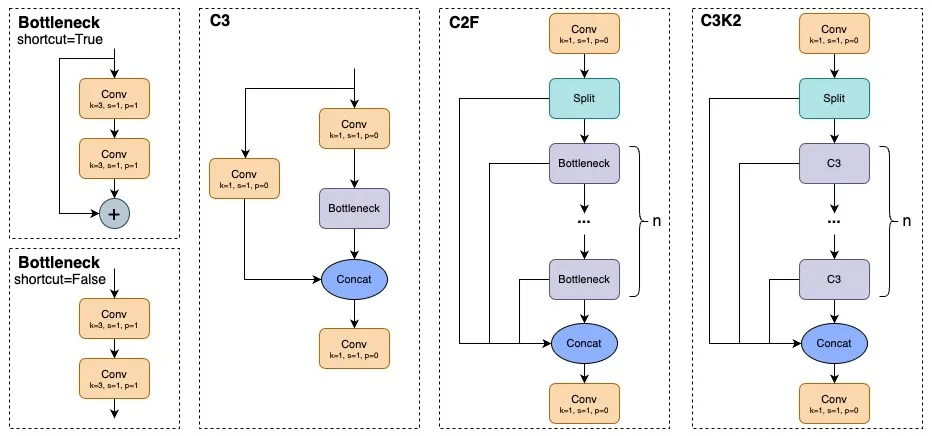
\includegraphics[scale=0.35]{gambar/C3k2.jpg}
  \caption{Modul Bottleneck, C3, C2F, dan C3K2}
  \label{fig:c3k2}
\end{figure}

Fitur input diubah pada lapisan \emph{feedforward} ke dalam ruang berdimensi lebih tinggi, sehingga hubungan non-linear yang kompleks dapat tertangkap dengan lebih stabil.

\subsection{MediaPipe}
\label{subsec:MediaPipe}

\emph{MediaPipe} adalah framework \emph{open-source} yang dikembangkan oleh Google untuk membangun pipeline pemrosesan media yang efisien, termasuk dalam pengolahan gambar dan video. Framework ini menyediakan berbagai modul yang dapat dimanfaatkan untuk aplikasi seperti deteksi wajah, pelacakan tangan, dan estimasi pose.

Kerangka kerja \emph{MediaPipe} menggunakan konsep "graph," di mana setiap node dalam graph berfungsi sebagai "calculator" yang menjalankan tugas spesifik, seperti deteksi objek, pelacakan pose, atau segmentasi gambar. Konfigurasi node-node ini dapat disesuaikan melalui \emph{GraphConfig}, yang mendefinisikan topologi dan fungsionalitas dari keseluruhan sistem.

\begin{figure}[H]
  \centering
  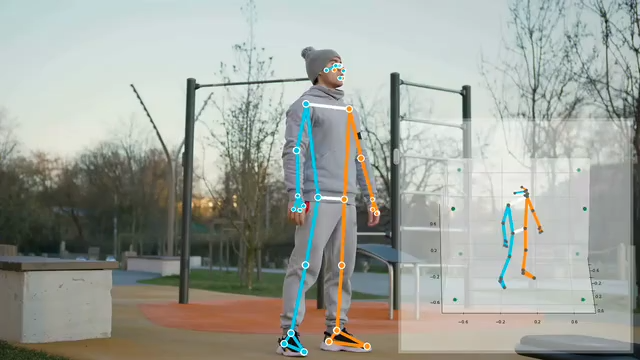
\includegraphics[scale=0.35]{gambar/MediaPipe3D.png}
  \caption{MediaPipe 3D.}
  \label{fig:MediaPipe3D}
\end{figure}

Salah satu contoh penggunaan \emph{MediaPipe} yang paling dikenal adalah estimasi pose manusia menggunakan modul \emph{MediaPipe Pose}. Teknik ini mengombinasikan estimasi pose 2D dengan model humanoid yang lebih kompleks, serta menggunakan metode optimasi untuk menghitung sudut sendi dalam pose 3D. Pendekatan ini efektif dalam mengatasi masalah ambiguitas kedalaman pada estimasi pose 3D, dan mampu bekerja secara \emph{real-time}. Visualisasi pose 3D yang dihasilkan memperlihatkan setiap sendi tubuh sebagai titik dan garis penghubung antar sendi, memberikan gambaran yang jelas mengenai posisi dan orientasi tubuh di dalam ruang 3D.

\subsubsection{MediaPipe Pose}
\label{subsubsec:MediaPipe Pose}

\emph{MediaPipe Pose} adalah modul dalam \emph{MediaPipe} yang dirancang khusus untuk mendeteksi dan melacak pose manusia secara \emph{real-time}. Dengan menggunakan model \emph{machine learning} yang canggih, \emph{MediaPipe Pose} dapat mengidentifikasi hingga 33 titik referensi pada tubuh manusia, memungkinkan sistem untuk memahami dan merespons gerakan pengguna secara cepat dan akurat.

\begin{figure}[H]
  \centering
  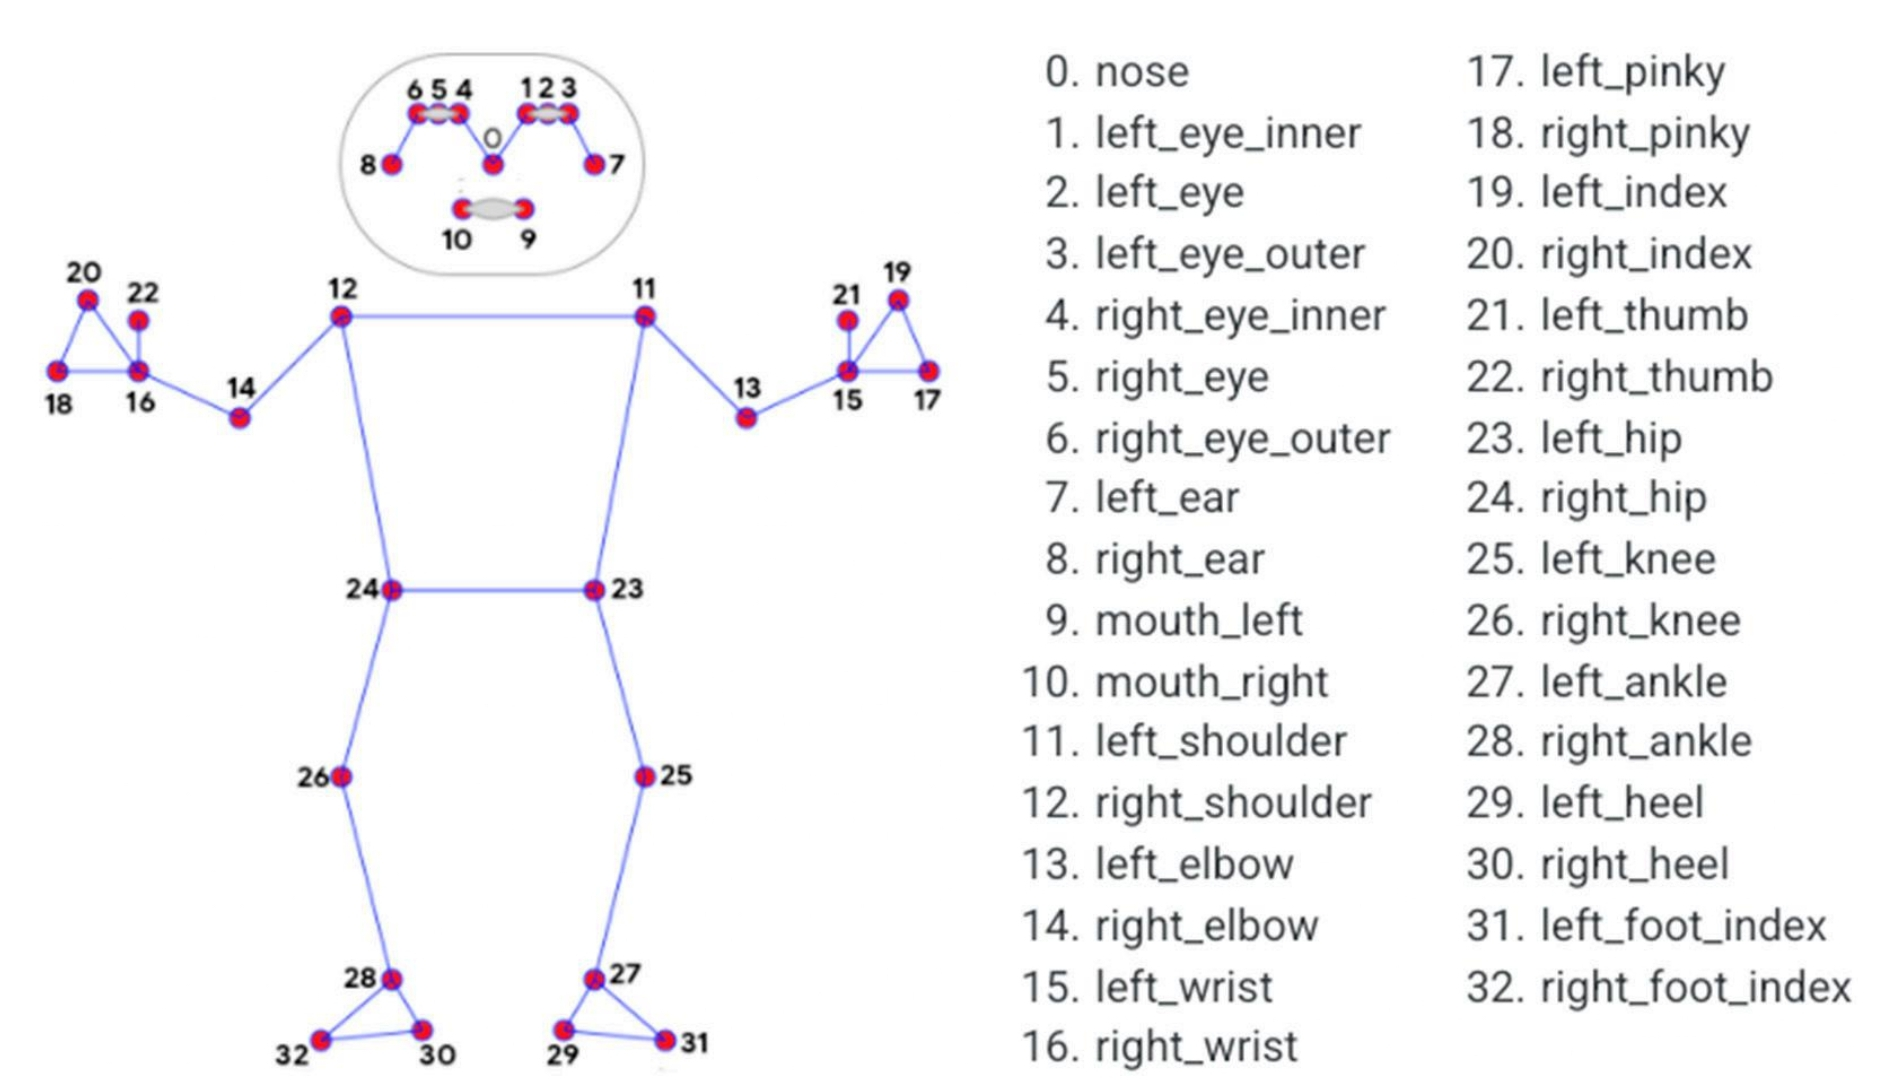
\includegraphics[scale=0.5]{gambar/mp_pose.jpg}
  \caption{MediaPipe Pose.}
  \label{fig:mp_pose}
\end{figure}

\subsection{Classification Performance}
\label{subsec:Classification Performance}

\emph{Classification performance} mengacu pada kemampuan model untuk mengklasifikasikan data input ke dalam kategori yang benar. Proses pengklasifikasian memerlukan evaluasi untuk menilai efektivitas model yang telah dikembangkan, biasanya dengan menggunakan set data pengetesan. Salah satu pendekatan evaluasi yang sering digunakan dalam konteks pengklasifikasian adalah \emph{confusion matrix}, yang memberikan visualisasi mengenai kinerja model dalam mengategorikan data secara akurat.

\begin{figure}[H]
  \centering
  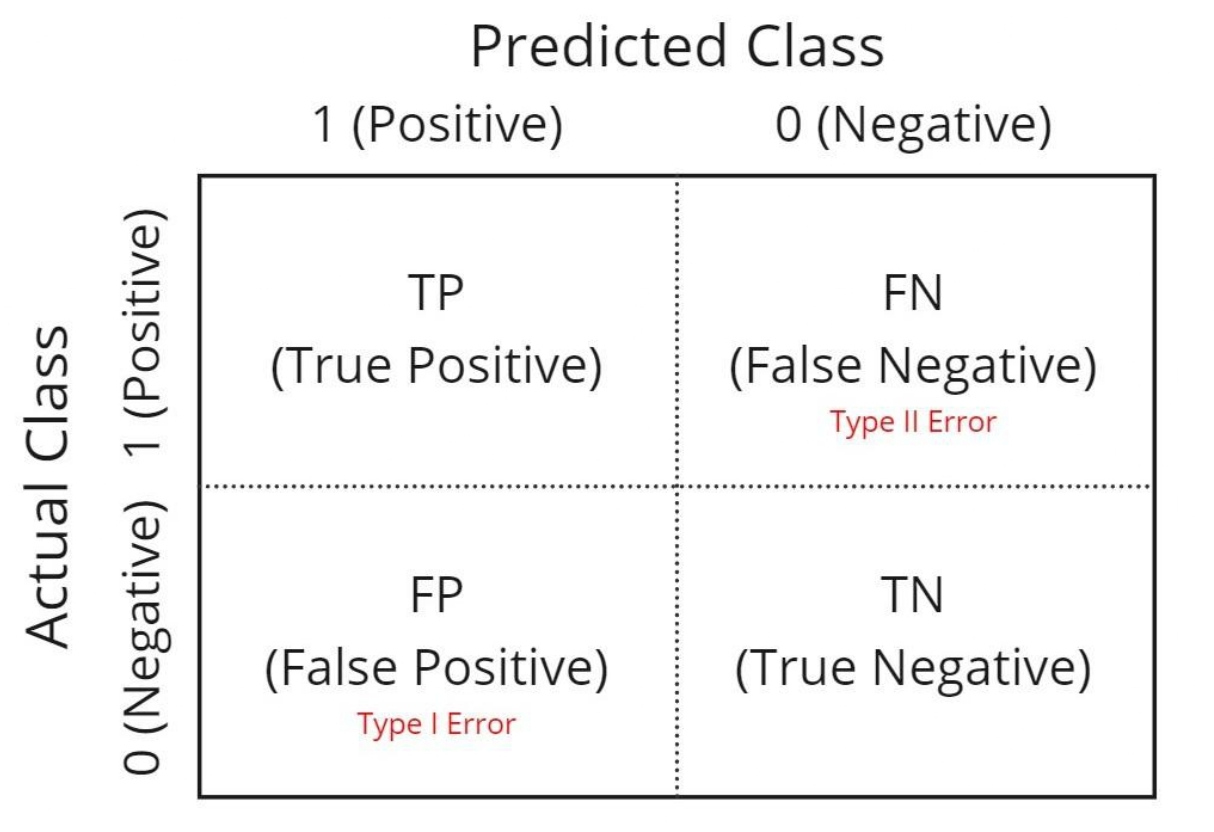
\includegraphics[scale=0.5]{gambar/Matrix Konfusi.jpg}
  \caption{Matrix Konfusi.}
  \label{fig:confusion}
\end{figure}

\emph{Confusion matrix} ini digunakan untuk mengevaluasi kinerja model klasifikasi biner dan menampilkan empat jenis hasil dari prediksi model: \emph{True Positive} (TP), \emph{False Negative} (FN), \emph{False Positive} (FP), dan \emph{True Negative} (TN). TP terjadi ketika model memprediksi kelas positif dengan benar, sedangkan FN terjadi ketika model salah memprediksi kelas negatif padahal seharusnya positif (disebut juga sebagai \emph{Type II Error}). FP terjadi ketika model salah memprediksi kelas positif padahal seharusnya negatif (disebut juga sebagai \emph{Type I Error}), dan TN terjadi ketika model memprediksi kelas negatif dengan benar.

\subsection{Evaluation Metrics}
\label{subsec:Evaluation Metrics}

Metrik evaluasi berfungsi sebagai dasar pemahaman dalam membandingkan efektivitas berbagai algoritma dan skenario yang berbeda. Melalui evaluasi yang teliti, perbandingan akurat antara berbagai teknik deteksi objek dapat dilakukan, serta tingkat keakuratan yang dicapai dapat dinilai dengan tepat. Hal ini menjadi sangat penting dalam pemilihan algoritma yang paling sesuai untuk tugas deteksi tertentu. Metrik seperti \emph{akurasi}, \emph{presisi}, dan \emph{recall} digunakan untuk mengevaluasi efektivitas model dalam mendeteksi dan mengidentifikasi objek dengan benar. Implementasi metrik-metrik ini diperlukan untuk menentukan model yang paling efisien.

Selain itu, analisis akurasi memberikan wawasan kuantitatif yang signifikan mengenai kinerja algoritma deteksi objek, serta detail lebih lanjut mengenai kemampuan algoritma dalam menghasilkan deteksi yang akurat. Kesalahan yang teridentifikasi melalui metrik evaluasi menjadi langkah penting dalam penelitian deteksi, seperti dalam kasus deteksi asap yang diteliti. Identifikasi ini memudahkan pemahaman mengenai potensi kesalahan dalam algoritma, yang kemudian dapat mengarah pada perbaikan dan peningkatan metode deteksi. Metrik evaluasi juga dimanfaatkan untuk mendukung pengoptimalan hiperparameter algoritma.

Dalam penelitian ini, berbagai metrik evaluasi seperti \emph{presisi}, \emph{recall}, dan \emph{Mean Average Precision} (mAP) telah diterapkan. Dengan menggabungkan metode evaluasi ini, penelitian ini dirancang untuk menyajikan analisis komprehensif mengenai kinerja algoritma deteksi objek yang ditinjau. Penjelasan mengenai konsep dasar metrik evaluasi akan dijabarkan sebagai berikut:

\subsubsection{Precision}
\label{subsubsec:precision}

\emph{Precision} merupakan salah satu metrik utama yang digunakan untuk mengukur seberapa akurat prediksi dari model terhadap objek yang terdeteksi. Metrik ini menunjukkan proporsi prediksi positif yang benar (\emph{True Positive}) dibandingkan dengan keseluruhan prediksi positif, baik yang benar (\emph{True Positive}) maupun salah (\emph{False Positive}), yang dinyatakan dengan persamaan berikut: 
\begin{equation} 
  \mathrm{Precision} = \frac{TP}{TP + FP} 
\end{equation}

Di mana \(TP\) (\emph{True Positive}): Prediksi benar, yaitu deteksi objek yang sesuai dengan \emph{ground truth} dan \(FP\) (\emph{False Positive}): Prediksi salah, yaitu deteksi objek yang tidak sesuai dengan \emph{ground truth}.

\emph{Precision} sangat berguna dalam situasi di mana kesalahan prediksi positif (\emph{false positive}) harus diminimalkan. Contohnya, dalam aplikasi kursi roda otonom, deteksi yang salah terhadap manusia dapat menyebabkan tindakan yang berbahaya, sehingga \emph{precision} harus dipertahankan pada nilai yang tinggi.

\emph{Precision} biasanya dikombinasikan dengan metrik lain, seperti \emph{recall}, untuk memberikan gambaran yang lebih lengkap tentang kinerja model.

\subsubsection{Recall}
\label{subsubsec:recall}

\emph{Recall} atau sensitivitas mengukur kemampuan model dalam mendeteksi semua objek yang ada pada gambar atau video. \emph{Recall} menekankan pada seberapa banyak objek yang benar-benar ada dalam data (\emph{ground truth}) yang berhasil terdeteksi oleh model dengan persamaan berikut:

\begin{equation} 
  \mathrm{Recall} = \frac{TP}{TP + FN} 
\end{equation}

Di mana \(TP\) (\emph{True Positive}): Prediksi benar, yaitu objek yang terdeteksi dengan benar dan \(FP\) (\emph{False Negative}): Prediksi salah, yaitu objek yang ada tetapi tidak terdeteksi.

Metrik ini penting ketika kesalahan berupa kegagalan dalam mendeteksi objek (\emph{false negative}) harus diminimalkan. Dalam konteks pengembangan kursi roda otonom, \emph{recall} sangat penting karena objek seperti manusia harus selalu terdeteksi agar kursi roda dapat mengikuti secara akurat.

\textbf{\emph{Trade-off Precision dan Recall:}} Dalam banyak kasus, \emph{precision} dan \emph{recall} memiliki hubungan yang berlawanan. Jika model terlalu konservatif dalam membuat prediksi, \emph{precision} akan tinggi, tetapi \emph{recall} rendah. Sebaliknya, jika model terlalu longgar dalam mendeteksi objek, \emph{recall} tinggi tetapi \emph{precision} menurun. Oleh karena itu, diperlukan keseimbangan antara \emph{precision} dan \emph{recall}, yang biasanya diekspresikan melalui metrik lain seperti \emph{F1-score}.

\subsubsection{Mean Average Precision (mAP)}
\label{subsubsec:mAP}

\emph{Mean Average Precision} (mAP) merupakan metrik komprehensif yang digunakan untuk mengukur performa model deteksi objek secara keseluruhan. \emph{mAP} adalah rata-rata dari \emph{average precision} (AP) di berbagai kelas yang ada dalam dataset.

\begin{equation} 
  \mathrm{AP} = \int_0^1 P(r) , dr 
\end{equation}

Di mana \(P(r)\) : \emph{Precision} sebagai fungsi dari \emph{recall} dan \(dr\) : Diferensial dari \emph{recall}.

AP dihitung dengan mencari area di bawah kurva \emph{precision-recall} (\emph{PR curve}) untuk setiap kelas. Setelah AP untuk semua kelas dihitung, rata-rata dari nilai-nilai tersebut akan memberikan nilai \emph{mAP}.

\begin{equation} 
  \mathrm{mAP} = \frac{1}{N} \sum_{i=1}^{N} \mathrm{AP}_i 
\end{equation}

Di mana \(N\) : Jumlah kelas dalam dataset dan \(AP_i\) : \emph{Average precision} untuk kelas ke-i.

\emph{mAP} memberikan gambaran yang lebih luas mengenai performa detektor objek, karena metrik ini mempertimbangkan baik \emph{precision} maupun \emph{recall} secara bersamaan. Nilai \emph{mAP} ini akan menjadi acuan untuk mengevaluasi performa sistem, seperti mendeteksi berbagai objek seperti manusia, rintangan, dan lingkungan sekitar.

\subsubsection{Intersection over Union (IoU)}
\label{subsubsec:IoU}

\emph{Intersection over Union} (\emph{IoU}) adalah metrik yang digunakan untuk mengevaluasi keakuratan deteksi posisi objek yang dilakukan oleh model dalam pemrosesan gambar. Area persinggungan antara kotak deteksi yang dihasilkan oleh model dan kotak referensi, yang dikenal sebagai \emph{Ground Truth}, dihitung untuk menilai kinerja model. Rasio ini diperoleh dengan membandingkan luas area irisan dari kedua kotak tersebut terhadap total luas area gabungan yang mereka cakup. Jika kedua kotak tersebut diperlakukan sebagai satu kesatuan, maka \emph{IoU} memberikan skor yang menunjukkan seberapa akurat model dalam memprediksi lokasi objek yang sebenarnya. Nilai \emph{IoU} akan semakin tinggi seiring dengan bertambahnya proporsi area persinggungan relatif terhadap keseluruhan area gabungan.

\begin{figure}[H]
  \centering
  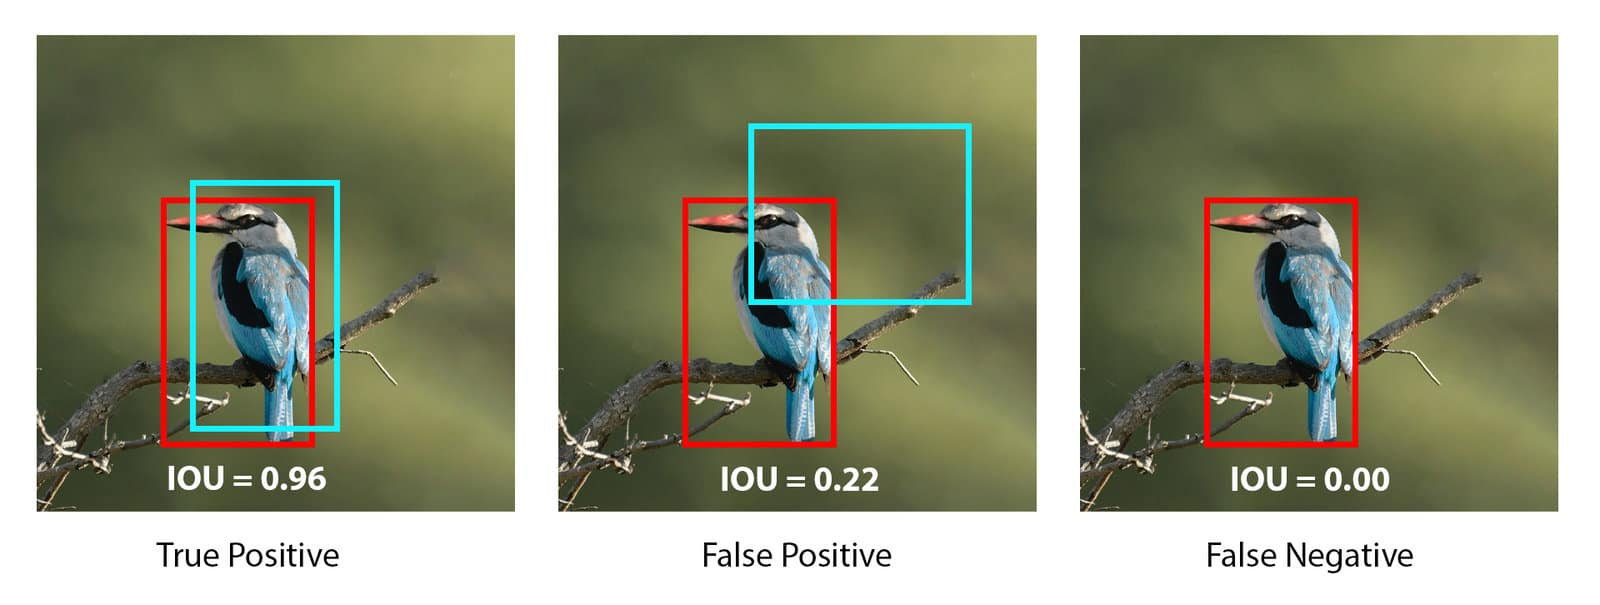
\includegraphics[scale=0.15]{gambar/IoU bbox.jpg}
  \caption{Intersection over Union.}
  \label{fig:IoU bbox}
\end{figure}

Kinerja model deteksi objek dilakukan evaluasi kinerja model deteksi objek dengan cara membandingkan area tumpang tindih antara \emph{bounding box} prediksi dan \emph{bounding box} \emph{ground truth}. Nilai \emph{IoU} berkisar antara 0 hingga 1, di mana nilai yang lebih mendekati 1 menunjukkan tingkat akurasi yang lebih tinggi dalam deteksi dan penentuan lokasi objek.

Dalam proses evaluasi, \emph{bounding box} yang dihasilkan oleh model dibandingkan dengan \emph{bounding box ground truth}, yang ditentukan secara manual sebagai lokasi sebenarnya dari objek dalam citra. Perhitungan \emph{IoU} dilakukan dengan membagi luas area tumpang tindih antara kedua \emph{bounding box} tersebut dengan luas total area gabungan dari keduanya. Persamaan berikut digunakan untuk menghitung nilai \emph{IoU}: 

\begin{equation}
  IoU = \frac{\left |A\bigcap B  \right |}{\left | A\bigcup B \right |}.
\end{equation}

\emph{IoU} dipilih sebagai alat ukur karena kemampuannya untuk memberikan penilaian yang jelas tentang seberapa akurat model dalam mengidentifikasi dan membatasi objek di berbagai kondisi, termasuk variasi ukuran, orientasi, dan konteks objek dalam citra. Nilai \emph{IoU} yang lebih tinggi diindikasikan sebagai tanda bahwa model dapat diandalkan dalam mendeteksi dan mengidentifikasi objek dengan tingkat presisi yang tinggi.

\subsection{Tinjauan Pustaka BoT-SORT}

BoT-SORT merupakan salah satu metode multi-object tracking (MOT) yang dikembangkan dengan pendekatan tracking-by-detection. Pada prinsipnya, metode ini memanfaatkan beberapa teknik dari berbagai algoritma sebelumnya, terutama ByteTrack, untuk menyajikan pelacakan yang lebih canggih. Perbaikan pada metode ini bertujuan untuk meningkatkan kinerja pelacakan dalam lingkungan dinamis maupun statis dengan memperbaiki beberapa komponen utama, yang akan dijabarkan sebagai berikut \cite{aharon2022botsortrobustassociationsmultipedestrian}:

\subsubsection{Kalman Filter}
\label{subsubsec:Kalman Filter}

Kalman Filter (KF) berfungsi untuk memprediksi lokasi objek di frame berikutnya berdasarkan pergerakan sebelumnya. BoT-SORT menggunakan KF dengan vektor status yang mencakup koordinat pusat objek ($x_c$, $y_c$), lebar ($w$), tinggi ($h$), dan laju perubahan (kecepatan) dari variabel-variabel tersebut ($\dot{x_c}$, $\dot{y_c}$, $\dot{w}$, $\dot{h}$) \cite{bewley2016simple, wojke2017simple}. Vektor status ini didefinisikan sebagai:

\begin{equation}
  \begin{split}
    \vb*{x}_k = [x_{c}{\scriptstyle(k)}, y_{c}{\scriptstyle(k)}, w{\scriptstyle(k)}, h{\scriptstyle(k)}, \\        
    \dot{x_{c}}{\scriptstyle(k)}, \dot{y_{c}}{\scriptstyle(k)}, \dot{w}{\scriptstyle(k)}, \dot{h}{\scriptstyle(k)}]^\top
  \end{split}
\end{equation}

\begin{equation}
  \vb*{z}_k = [z_{x_c}{\scriptstyle(k)}, z_{y_c}{\scriptstyle(k)}, z_{w}{\scriptstyle(k)}, z_{h}{\scriptstyle(k)}]^\top
\end{equation}

Matriks noise proses ($\mathbf{Q}_k$) dan noise pengukuran ($\mathbf{R}_k$) disesuaikan agar lebih sensitif terhadap perubahan dalam frame, yang membantu meningkatkan akurasi pelacakan. Matriks $\mathbf{Q}_k$ dan $\mathbf{R}_k$ ditentukan sebagai berikut:

\begin{equation}
  \begin{split}
    \vb*{Q}_k = diag\big{(} (\sigma_{p} \hat{w}_{k-1|k-1})^2, (\sigma_{p} \hat{h}_{k-1|k-1})^2, \\
    (\sigma_{p} \hat{w}_{k-1|k-1})^2, (\sigma_{p} \hat{h}_{k-1|k-1})^2, \\
    (\sigma_{v} \hat{w}_{k-1|k-1})^2, (\sigma_{v} \hat{h}_{k-1|k-1})^2, \\ 
    (\sigma_{v} \hat{w}_{k-1|k-1})^2 ,(\sigma_{v} \hat{h}_{k-1|k-1})^2\big{)}
  \end{split}
\end{equation}

\begin{equation}
  \begin{split}
      \vb*{R}_k = diag\big{(}(\sigma_{m} \hat{w}_{k|k-1})^2, (\sigma_{m} \hat{h}_{k|k-1})^2, \\
      (\sigma_{m} \hat{w}_{k|k-1})^2, (\sigma_{m} \hat{h}_{k|k-1})^2\big{)} 
  \end{split}
\end{equation}

Dengan adanya perubahan ini, prediksi \emph{bounding box} lebih akurat dibandingkan dengan metode Kalman Filter tradisional, terbukti dengan peningkatan nilai HOTA (Higher Order Tracking Accuracy).

\begin{figure}[H]
  \centering
  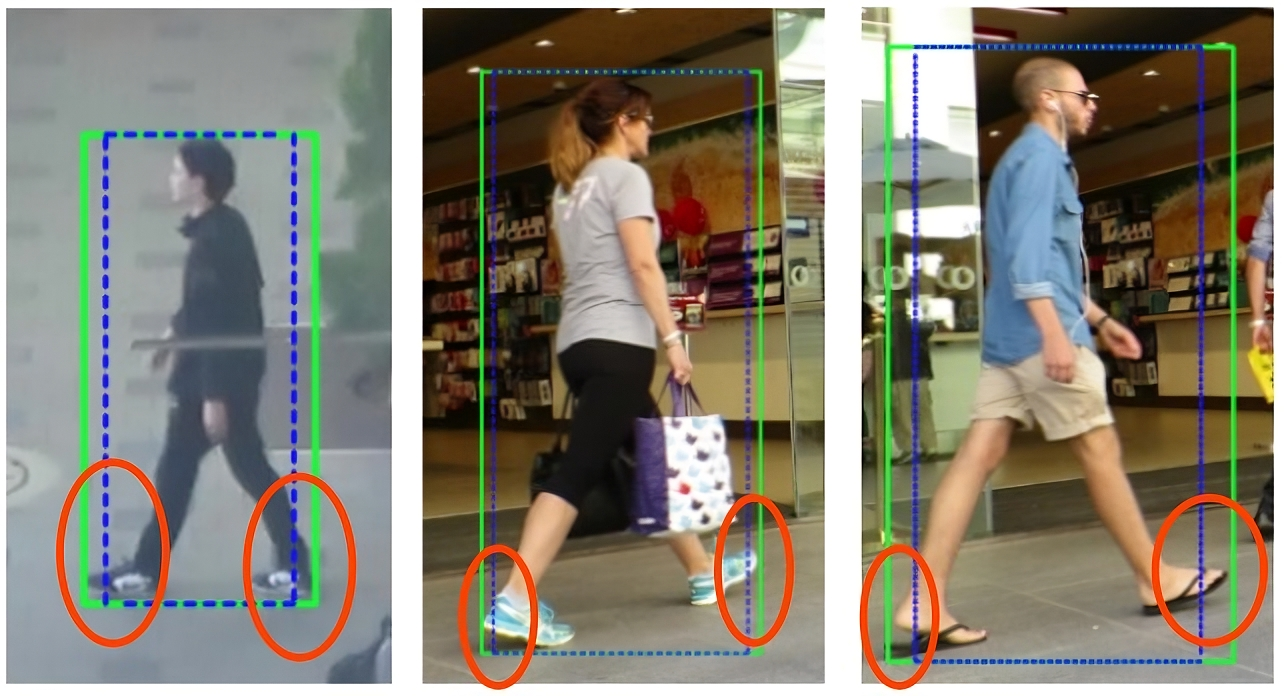
\includegraphics[scale=0.19]{gambar/KF_width.png}
  \caption{Kalman Filter bbox.}
  \label{fig:KF width}
\end{figure}

Visualisasi bentuk \emph{bounding box} dibandingkan dengan \emph{Kalman filter} yang banyak digunakan~\cite{wojke2017simple} (biru putus-putus) dan \emph{Kalman filter} yang diusulkan (hijau). Tampak bahwa lebar \emph{bounding box} yang dihasilkan oleh \emph{Kalman filter} yang diusulkan lebih sesuai dengan objek. \emph{Bounding box} biru putus-putus memotong bagian kaki objek (dalam merah), sedangkan \emph{bounding box} hijau mencapai lebar yang diinginkan.

\subsubsection{\emph{Camera Motion Compensation} (CMC)}
\label{subsubsec:Camera Motion Compensation}

Pelacak berbasis tracking-by-detection seringkali mengalami masalah ID switch atau false negatives akibat gerakan kamera, terutama dalam situasi dinamis. BoT-SORT mengimplementasikan teknik kompensasi gerakan kamera (Camera Motion Compensation) dengan memanfaatkan affine transformation untuk menghitung transformasi antara dua frame. Dengan melakukan ekstraksi keypoints gambar \cite{shi1994good}, kemudian menggunakan sparse optical flow ~\cite{Bouguet1999PyramidalIO} untuk pelacakan fitur dengan penolakan outlier lokal berbasis translasi. Matriks affine $\vb*{A}_{k-1}^k\in \mathbb{R}^{2 \times 3}$ diselesaikan menggunakan metode RANSAC ~\cite{fischler1981random}. Penggunaan teknik pendaftaran spars memungkinkan pengabaian objek dinamis dalam adegan berdasarkan deteksi, sehingga memiliki potensi untuk memperkirakan gerakan latar belakang dengan lebih akurat.

\begin{equation}
  \begin{aligned}
      & \vb*{A}_{k-1}^k = 
      \begin{bmatrix}
          \vb*{M}_{2x2} | \vb*{T}_{2x1}
      \end{bmatrix} = 
      \begin{bmatrix}
          a_{11}\;a_{12}\;a_{13} \\ a_{21}\;a_{22}\;a_{23} \\ 
      \end{bmatrix}
  \end{aligned}
\end{equation}
\begin{equation}
  \begin{aligned}
  {
      \vb*{\tilde{M}}}^k_{k-1} = 
      \begin{bmatrix}
      \vb*{M} & \vb*{0} & \vb*{0} & \vb*{0} \\
      \vb*{0} & \vb*{M} & \vb*{0} & \vb*{0} \\
      \vb*{0} & \vb*{0} & \vb*{M} & \vb*{0} \\
      \vb*{0} & \vb*{0} & \vb*{0} & \vb*{M}
      \end{bmatrix}, \; 
      \tilde{\vb*{T}}_{k-1}^k = 
      \begin{bmatrix}a_{13}\\a_{23}\\ 0\\ 0\\ \vdots \\ 0\end{bmatrix}
  \end{aligned}
\end{equation}
\begin{equation}
  \begin{aligned}
      \hat{\vb*{x}}^\prime_{k|k-1} = \tilde{\vb*{M}}_{k-1}^k \hat{\vb*{x}}_{k|k-1} + \tilde{\vb*{T}}_{k-1}^k \\
  \end{aligned}
\end{equation}
\begin{equation}
    {{\vb*{P}}}^{\prime}_{k|k-1} = 
    \tilde{\vb*{M}}_{k-1}^k {\vb*{P}}_{k|k-1} {\tilde{\vb*{M}}_{k-1}}^{k^\top}
    \label{eq:cmc_cov}        
\end{equation}

Dimana $\vb*{M}\in \mathbb{R}^{2 \times 2}$ merupakan matriks yang berisi skala dan rotasi dari matriks afine $\vb*{A}$, dan $T$ mengandung komponen translasi. Trik matematis digunakan dengan mendefinisikan $\tilde{\vb*{M}}^k_{k-1}\in \mathbb{R}^{8 \times 8}$ dan $\tilde{\vb*{T}}_{k-1}^k\in \mathbb{R}^{8}$. Selanjutnya, $\hat{\vb*{x}}_{k|k-1}$ dan $\hat{\vb*{x}}^\prime_{k|k-1}$ didefinisikan sebagai vektor status prediksi dari Kalman Filter (KF) pada waktu $k$, sebelum dan setelah kompensasi gerakan kamera, sedangkan $\vb*{P}_{k|k-1}$ dan $\vb*{P'}_{k|k-1}$ didefinisikan sebagai matriks kovarians KF sebelum dan setelah koreksi. Setelah itu, $\hat{\vb*{x}}^\prime_{k|k-1}$ dan ${{\hat{\vb*{P}}}^{\prime}}_{k|k-1}$ digunakan dalam langkah update Kalman Filter sebagai berikut.

\begin{equation}
  \begin{aligned}
  & \vb*{K_k} =  {{\vb*{P}}}^{\prime}_{k|k-1} \vb*{H}_k^\top (\vb*{H}_k  {{\vb*{P}}}^{\prime}_{k|k-1} \vb*{H}_k^\top + \vb*{R}_k)^{-1} \\
  & \hat{\vb*{x}}_{k|k} = \hat{\vb*{x}}^\prime_{k|k-1} + \vb*{K}_k (\vb*{z}_k - \vb*{H}_k \hat{\vb*{x}}^\prime_{k|k-1}) \\
  & \vb*{P}_{k|k} = (\vb*{I}- \vb*{K}_k \vb*{H}_k)  {{\vb*{P}}}^{\prime}_{k|k-1}
  \end{aligned}
  \label{eq:cmc_update_kf}
\end{equation} 

Dalam skenario kecepatan tinggi, koreksi penuh terhadap vektor status, termasuk komponen kecepatan, sangat penting. Jika kamera berubah dengan lambat dibandingkan dengan kecepatan frame, koreksi pada persamaan \ref{eq:cmc_cov} dapat diabaikan. Setelah mengompensasi gerakan kamera yang rigid dan dengan asumsi posisi objek hanya sedikit berubah dari satu frame ke frame berikutnya, pada aplikasi dengan frame rate tinggi, ketika deteksi hilang, prediksi lintasan dapat dilakukan menggunakan langkah prediksi KF, yang memungkinkan tampilan lintasan yang lebih kontinu dan MOTA yang lebih tinggi.

Visualisasi prediksi \emph{bounding box} (BB) dari tracklet digunakan untuk asosiasi dengan BB deteksi baru berdasarkan kriteria IoU maksimum. (a.1) dan (b.1) memperlihatkan prediksi dari Kalman Filter (KF). (a.2) dan (b.2) memperlihatkan prediksi dari KF setelah kompensasi gerakan kamera. Pada gambar (b.1), diperlihatkan skenario di mana pengabaian gerakan kamera dapat menyebabkan IDSWs atau FN. Sebaliknya, pada gambar (b.2), prediksi telah sesuai dengan lokasi yang diinginkan dan asosiasi berhasil dilakukan. Gambar \ref{fig:cmc} dihasilkan dari sekuens MOT17 \cite{milan2016mot16}, yang mencakup pergerakan kamera akibat manuver kendaraan yang berbelok ke arah kanan.

\begin{figure}[H]
  \centering
  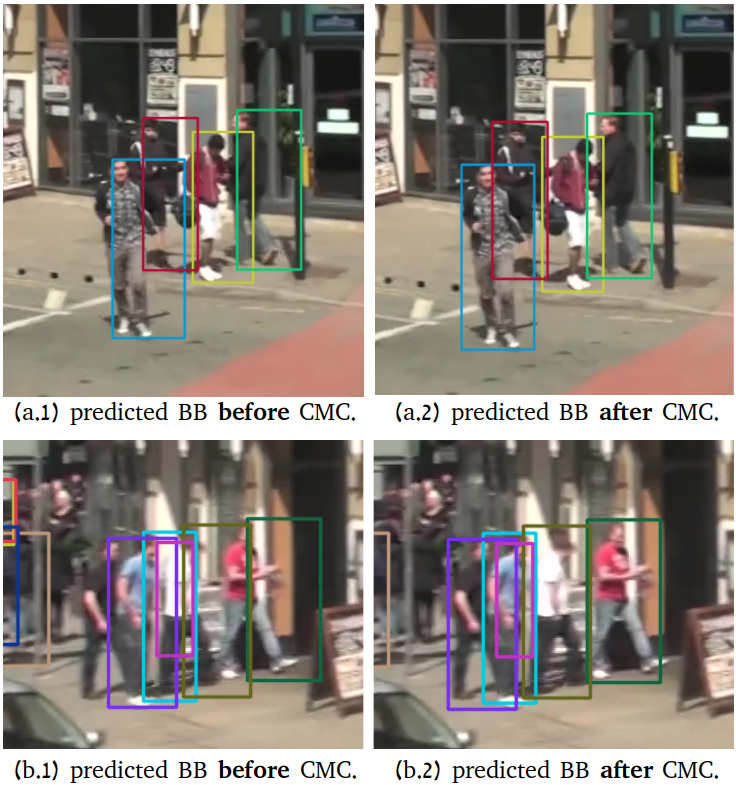
\includegraphics[scale=0.33]{gambar/cmc_pred.png}
  \caption{Kompensasi Gerakan Kamera}
  \label{fig:cmc}
\end{figure}

\subsubsection{Fusi IoU - Re-ID}
\label{subsubsec:Fusi IoU - Re-ID}

Fitur Re-ID diintegrasikan untuk memanfaatkan kemajuan dalam representasi visual objek. Fitur Re-ID diekstraksi menggunakan FastReID dengan backbone ResNeSt50 \cite{he2020fastreid, zhang2020resnest}, dan mekanisme exponential moving average (EMA) digunakan untuk memperbarui status appearance tracklet \cite{wang2020towards}. Pembaruan status appearance dilakukan dengan rumus:

\begin{equation}
e_i^k = \alpha e_i^{k-1} + (1 - \alpha) f_i^k
\end{equation}

Di mana $e_i^k$ adalah status appearance untuk tracklet ke-$i$ pada frame $k$, $f_i^k$ adalah embedding appearance deteksi saat ini, dan $\alpha=0.9$ adalah momentum term.

Penggabungan antara informasi gerakan (IoU) dan appearance (cosine similarity) dilakukan dengan cara berikut. Pertama, kandidat dengan kesamaan cosinus rendah atau yang terlalu jauh berdasarkan skor IoU ditolak. Selanjutnya, nilai minimum pada setiap elemen matriks digunakan sebagai nilai akhir dari \emph{cost matrix} $C$. Pipeline fusi IoU-ReID ini dapat diformulasikan sebagai berikut:

\begin{equation}
  \begin{aligned}
  & \hat{d}_{i, j}^{cos} = 
    \begin{cases}
      0.5 \cdot d_{i, j}^{cos}, \text{($d_{i, j}^{cos} < \theta_{emb})$ $\land$ $(d_{i, j}^{iou} < \theta_{iou})$}\\
      1, \text{otherwise}
    \end{cases} \\
  \end{aligned}
  \label{eq:min_dist}        
\end{equation}

\begin{equation}
  C_{i, j} = \min\{d_{i, j}^{iou}, \hat{d}_{i, j}^{cos}\}
\end{equation}

\begin{equation}
  \begin{aligned}
  \hat{b} = 
    \begin{cases}
      0, \quad\quad \Delta data \neq 0 \\
      1, \quad \neg ( \hat{t} \in [0, t] \lor b ) \\
      b, \quad\quad \text{otherwise}\\
    \end{cases}
  \end{aligned}       
\end{equation}

Di mana $C_{i, j}$ merupakan elemen $(i, j)$ dari \emph{cost matrix} $C$. $d_{i, j}^{iou}$ adalah jarak IoU antara prediksi \emph{bounding box} tracklet ke-$i$ dan \emph{bounding box} deteksi ke-$j$, yang merepresentasikan \emph{cost} gerakan. $d_{i, j}^{cos}$ adalah jarak cosinus antara deskriptor penampilan rata-rata tracklet ke-$i$ dan deskriptor deteksi baru ke-$j$. $\hat{d}_{i, j}^{cos}$ adalah \emph{cost} penampilan baru yang digunakan. $\theta_{iou}$ adalah \emph{threshold} kedekatan, yang ditetapkan sebesar 0.5, untuk menolak pasangan tracklet dan deteksi yang tidak mungkin. $\theta_{emb}$ adalah \emph{threshold} penampilan, yang digunakan untuk memisahkan asosiasi positif dari keadaan penampilan tracklet dan vektor embedding deteksi dari asosiasi negatif.
Permasalahan penugasan linear dari deteksi dengan \emph{confidence} tinggi, yaitu langkah asosiasi pertama, diselesaikan menggunakan algoritma Hungarian~\cite{kuhn1955hungarian} dan berdasarkan \emph{cost matrix} $C$, yang dibentuk menggunakan Persamaan~\ref{eq:min_dist}.

\subsection{\emph{RoboFlow}}
\label{subsec:RoboFlow}

\emph{RoboFlow} adalah platform yang mendukung pengolahan data secara efisien dan efektif. Melalui berbagai fitur yang disediakan, mulai dari anotasi data hingga evaluasi model, \emph{RoboFlow} memastikan bahwa setiap tahap dalam alur kerja pembelajaran mesin dapat dilakukan dengan lebih terstruktur dan mudah diintegrasikan dengan kerangka kerja yang ada. Peningkatan kinerja model dapat dikembangkan tanpa terbebani oleh kompleksitas teknis dalam penyiapan data.

\emph{RoboFlow} memfasilitasi proses penandaan gambar melalui alat bantu intuitif, sehingga percepatan dalam pembuatan label untuk \emph{dataset} dapat tercapai. Gambar dalam \emph{dataset} secara otomatis dimodifikasi melalui augmentasi data untuk menciptakan variasi guna meningkatkan \emph{robustness} model yang dilatih. Dukungan untuk konversi antara berbagai format \emph{dataset} populer juga disediakan, memudahkan persiapan data untuk berbagai algoritma pembelajaran mesin. Selain itu, fungsi untuk membagi \emph{dataset} menjadi set pelatihan, validasi, dan pengujian untuk validasi model.

\emph{RoboFlow} juga menawarkan integrasi dengan banyak kerangka kerja pembelajaran mesin populer seperti \emph{TensorFlow}, \emph{PyTorch}, dan \emph{YOLO}, yang mencakup:

\begin{itemize}
    \item \emph{Ekspor Data}: \emph{Dataset} dapat dengan mudah diekspor dalam format yang siap digunakan oleh kerangka kerja pembelajaran mesin.
    \item \emph{Pelatihan Model}: Platform ini memungkinkan pelatihan model secara langsung menggunakan \emph{dataset} yang telah disiapkan dan dioptimalkan.
    \item \emph{Evaluasi Model}: Kinerja model diukur menggunakan metrik yang membantu dalam memahami dan menyesuaikan efektivitas model sesuai kebutuhan.
\end{itemize}

\subsection{OBS Studio}
\label{subsec:OBS Studio}

\emph{OBS Studio} adalah perangkat lunak \emph{open-source} yang dirancang untuk streaming dan perekaman video. Dalam proyek ini, \emph{OBS Studio} digunakan untuk mendokumentasikan dan menganalisis performa kursi roda otonom selama fase pengujian. Perangkat lunak ini memungkinkan pemilihan berbagai sumber video input, termasuk \emph{webcam}, yang digunakan untuk merekam seluruh proses pengujian secara visual. Dengan \emph{OBS Studio}, proses pengujian dari awal hingga akhir dapat direkam secara lengkap, memungkinkan pengumpulan data visual yang kaya dan mendetail.

\subsection{ESP32 Devkit V1}
\label{subsec:ESP32 Devkit V1}

\emph{ESP32 Devkit V1} adalah sebuah mikrokontroler yang dilengkapi dengan kemampuan komunikasi nirkabel, termasuk \emph{Wi-Fi} dan \emph{Bluetooth}. Dalam proyek ini, \emph{ESP32 Devkit V1} digunakan sebagai modul komunikasi utama untuk kursi roda otonom. Perangkat ini memungkinkan kursi roda untuk berinteraksi dengan perangkat eksternal seperti \emph{smartphone} atau komputer melalui jaringan nirkabel.

Salah satu keunggulan utama dari \emph{Devkit} ini adalah banyaknya pin yang dimiliki, yang memungkinkan mikrokontroler untuk diprogram dengan berbagai tugas. Pin-pin ini memberikan fleksibilitas yang tinggi dalam menghubungkan berbagai sensor dan aktuator yang diperlukan. Dengan memanfaatkan berbagai pin tersebut, sistem dapat menjalankan beberapa tugas secara simultan, seperti mengumpulkan data dari sensor, mengontrol motor, dan mengelola komunikasi nirkabel.

\begin{figure}[H]
  \centering
  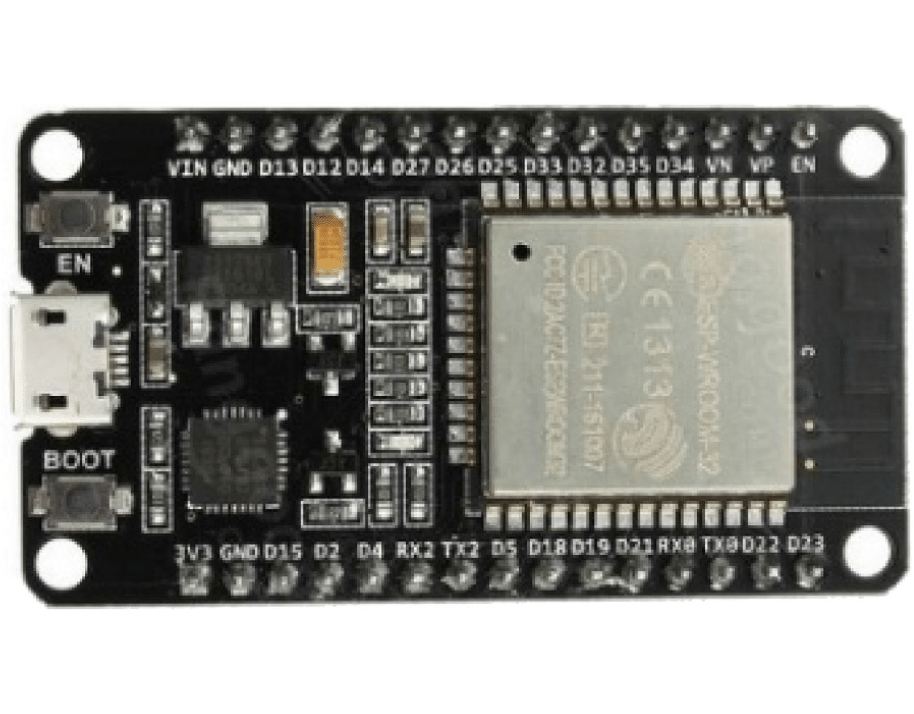
\includegraphics[scale=0.25]{gambar/ESP32-DEVKIT-V1-board.png}
  \caption{Gambar ESP32 Devkit V1}
  \label{fig:Gambar ESP32Devkit V1}
\end{figure}

\emph{Devkit} ini kompatibel dengan \emph{Arduino IDE} dengan bahasa pemrograman \emph{C++}, yang merupakan platform yang umum digunakan. \emph{Arduino IDE} menyediakan berbagai \emph{library} dan dukungan yang memudahkan proses pemrograman \emph{ESP32} untuk mengontrol berbagai perangkat keras yang terhubung. Dengan pemrograman dalam \emph{C++}, kode yang efisien dan terstruktur dapat dihasilkan untuk menjalankan berbagai tugas kompleks, seperti pemrosesan data sensor dan pengendalian motor.

\subsection{Motor Driver H-Bridge}
\label{subsec:Motor}

\emph{Motor Driver H-Bridge} adalah komponen elektronik yang krusial dalam pengendalian motor \emph{DC} pada kursi roda. Komponen ini memungkinkan pengaturan arah dan kecepatan motor, yang esensial untuk navigasi kursi roda dalam berbagai kondisi. Dengan memanfaatkan \emph{H-Bridge}, motor pada kursi roda dapat digerakkan maju, mundur, atau berbelok sesuai dengan kebutuhan.

\begin{figure}[H]
  \centering
  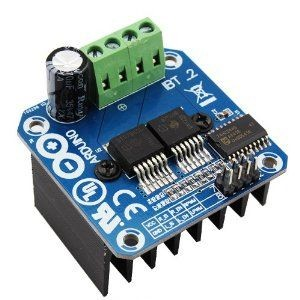
\includegraphics[scale=0.4]{gambar/Motor Driver H - bridge Bts.jpg}
  \caption{Gambar Motor Driver H-Bridge}
  \label{fig:Gambar Motor Driver H-Bridge}
\end{figure}

Penggunaan \emph{H-Bridge} dalam sistem otonom memungkinkan penyesuaian gerakan kursi roda secara \emph{real-time} berdasarkan informasi yang diterima dari sensor. Hal ini memungkinkan kursi roda untuk mengikuti gerakan pengguna dengan presisi tinggi. Kemampuan untuk menavigasi secara mandiri menjadi sangat penting dalam memastikan bahwa kursi roda dapat beroperasi dengan aman dan efisien di berbagai lingkungan.

\subsection{Kursi Roda Elektrik KY-123}
\label{subsec:KY-123}

Kursi roda elektrik \emph{KY-123} digunakan sebagai platform utama dalam pengembangan kursi roda otonom dalam penelitian ini. Kursi roda ini dilengkapi dengan motor dan kontroler yang telah terintegrasi, yang memungkinkan modifikasi lebih lanjut untuk mendukung sistem otonom yang dirancang.

Dengan penambahan sensor, kamera, dan perangkat keras lainnya, kursi roda \emph{KY-123} diharapkan dapat menjalankan fungsi otonom, termasuk kemampuan untuk mengikuti pergerakan pengguna secara mandiri. Pengintegrasian antara perangkat keras dan perangkat lunak pada \emph{KY-123} menjadi elemen kunci dalam mencapai sistem yang handal dan efektif. Modifikasi ini bertujuan untuk meningkatkan mobilitas dan kemudahan penggunaan bagi individu dengan keterbatasan fisik, serta memastikan performa yang optimal dalam berbagai skenario penggunaan.

\begin{figure}[H]
  \centering
  \includegraphics[scale=0.05]{gambar/kursi roda.png}
  \caption{Gambar Kursi Roda Elektrik KY-123}
  \label{fig:Gambar Kursi Roda Elektrik KY-123}
\end{figure}
% Ubah judul dan label berikut sesuai dengan yang diinginkan.
\section{Desain dan Implementasi}
\label{sec:desaindanimplementasi}

\subsection{Deskripsi Sistem}
\label{subsec:deskripsisistem}

Pada tahap ini, kursi roda otonom dikembangkan untuk dapat mengikuti manusia menggunakan algoritma deteksi berbasis YOLOv11. Sistem ini dirancang dengan tujuan utama meningkatkan mobilitas pengguna yang membutuhkan bantuan dalam bergerak. Sistem terdiri dari komponen perangkat keras dan perangkat lunak, yang terintegrasi untuk mencapai tujuan ini.

\subsubsection{Komponen Sistem}
\label{subsubsec:komponensistem}

Sistem ini terdiri dari:

\begin{itemize}
    \item \textbf{VS Code}: Digunakan sebagai lingkungan pengembangan untuk menjalankan kode terkait YOLOv11 dan analisis lainnya.
    \item \textbf{Arduino IDE}: Mengembangkan dan mengunggah kode ke ESP32 yang mengendalikan motor dan sensor.
    \item \textbf{Laptop}: Berfungsi sebagai pusat pemrosesan data yang lebih kompleks dan pengembangan perangkat lunak.
    \item \textbf{Kamera (OV5640 5MP)}: Menangkap gambar lingkungan secara real-time dan mendeteksi target (manusia) menggunakan YOLOv11.
    \item \textbf{ESP32 Devkit V1}: Berfungsi sebagai pengontrol utama yang mengelola data dari kamera dan mengendalikan pergerakan kursi roda.
    \item \textbf{2 Kontroller Motor}: Mengendalikan motor DC yang menggerakkan kursi roda.
    \item \textbf{2 DC-DC Voltage Regulator}: Mengatur tegangan untuk komponen elektronik agar tetap stabil.
    \item \textbf{2 Motor DC}: Menggerakkan kursi roda, dikontrol melalui driver motor yang menerima sinyal dari mikroprosesor.
    \item \textbf{Baterai 24V}: Sebagai sumber daya utama untuk keseluruhan sistem, termasuk mikroprosesor, motor, dan perangkat lainnya.
\end{itemize}

\subsubsection{Arsitektur Sistem}
\label{subsubsec:arsitektursistem}

Arsitektur sistem dirancang agar kamera menangkap gambar secara terus-menerus, kemudian mengirimkan data ke mikroprosesor ESP32 untuk diproses. YOLOv11 digunakan untuk mendeteksi manusia dan memberikan informasi koordinat posisi target. Informasi ini kemudian digunakan oleh mikroprosesor untuk mengontrol motor dan mengarahkan kursi roda agar dapat mengikuti pergerakan target secara dinamis.

\subsection{Perangkat Keras}
\label{subsec:perangkathardware}

Desain perangkat keras melibatkan integrasi antara beberapa komponen yang disebutkan sebelumnya. Kamera dipasang di bagian depan kursi roda untuk mendapatkan sudut pandang optimal terhadap target. Mikroprosesor ESP32 ditempatkan di bagian bawah kursi roda bersama dengan driver motor dan baterai untuk menjaga keseimbangan.

\begin{itemize}
    \item \textbf{Unit Kontrol}: Unit Kontrol seperti komputer atau laptop digunakan sebagai pusat pemrosesan utama untuk menjalankan YOLOv11 dan mediapipe, menganalisis hasil deteksi dan menghasilkan keputusan berupa kode instruksi.
    \item \textbf{Kamera OV5640}: Kamera ini terhubung ke ESP32 untuk menangkap frame dengan menggunakan sensor 5MP.
    \item \textbf{ESP32}: Microcontroller ini menerima data dari kamera dan kemudian menjalankan algoritma untuk diproses pada komputer, lalu mengirim sinyal kontrol ke driver motor.
    \item \textbf{Driver Motor L298N}: Driver ini digunakan untuk mengontrol kecepatan dan arah putaran motor DC yang menggerakkan kursi roda.
\end{itemize}

\subsubsection{Kamera}
\label{subsubsec:kamera}
Kamera yang digunakan dalam sistem ini adalah OV5640, sebuah sensor kamera CMOS (Complementary Metal-Oxide-Semiconductor) dengan resolusi 5 megapiksel (MP). Sensor ini memiliki kemampuan menangkap gambar hingga resolusi maksimum 2592x1944 piksel, yang memberikan hasil citra dengan detail yang sangat baik. Sensor ini mendukung pengambilan gambar dan video secara real-time, dengan frame rate mencapai 30 frame per detik (fps) pada resolusi 1080p, sehingga ideal untuk aplikasi yang memerlukan pengolahan citra secara langsung.

Selain resolusinya yang tinggi, OV5640 juga dilengkapi dengan berbagai fitur canggih untuk pengolahan gambar otomatis. Berdasarkan datasheet, fitur seperti auto white balance, auto exposure, dan auto focus memungkinkan kamera ini beradaptasi secara otomatis terhadap perubahan kondisi pencahayaan dan jarak, sehingga tetap menghasilkan gambar berkualitas tinggi dalam berbagai situasi. OV5640 juga mendukung fitur face detection dan image scaling, yang sangat berguna dalam mendeteksi objek atau target manusia secara cepat dan akurat.

\subsubsection{Unit Kontrol}
\label{subsubsec:UnitKontrol}
% Pada sistem ini, unit kontrol utama yang digunakan adalah laptop pribadi yang berperan sebagai pengolah data utama selama pengujian. Laptop ini memiliki spesifikasi yang dirancang untuk menangani beban komputasi tinggi, sangat cocok untuk pengolahan data secara real-time, sebagaimana ditunjukkan pada tabel.

% \begin{table}[H]
%   \centering
%   \caption{Spesifikasi Laptop MSI GF63 untuk Unit Kontrol}
%   \begin{tabular}{|l|l|}
%   \hline
%   \textbf{Komponen}       & \textbf{Spesifikasi}                     \\ \hline
%   Model Laptop            & MSI GF63                                 \\ \hline
%   Prosesor                & Intel Core i7-10750H, 6 core, 12 threads \\ \hline
%   GPU                     & NVIDIA RTX 3050                          \\ \hline
%   RAM                     & 16GB DDR4, 3200 MHz                      \\ \hline
%   Penyimpanan             & SSD M.2                                  \\ \hline
%   Konektivitas WiFi       & WiFi 802.11ac (MU-MIMO)                  \\ \hline
%   Pengolahan Data         & Inferensi model, ESP dan Python (venv)   \\ \hline
%   \end{tabular}
% \end{table}

Unit kontrol pada sistem ini, berperan sebagai pengolah data utama selama pengujian, dengan spesifikasi yang dirancang untuk menangani beban komputasi tinggi dan cocok untuk pengolahan data secara real-time.

Salah satu aspek penting dari unit kontrol dalam proyek ini adalah dukungan WiFi yang cepat dan stabil dalam komunikasi antar perangkat. Sistem bergantung pada data video yang dikirim oleh kamera OV5640 melalui ESP32 ke laptop untuk diolah, dan proses ini harus berlangsung tanpa hambatan. Konektivitas WiFi yang disediakan juga memungkinkan pengiriman data dalam waktu nyata dengan minim latensi, yang sangat penting untuk deteksi target secara cepat.

Kemampuan untuk menjaga kestabilan koneksi WiFi pada jarak yang lebih jauh dari router juga penting dalam pengujian di area yang luas. Seperti dengan menangani beberapa perangkat yang terhubung secara simultan, memungkinkan komunikasi yang efisien antara ESP32 tanpa penurunan performa. Teknologi ini sangat penting untuk memastikan bahwa sistem dapat terus memproses data video yang dikirimkan oleh kamera dan memberikan instruksi dengan respons yang cepat.

Data citra yang didapatkan menggunakan kamera OV5640, selanjutnya akan diproses melalui serangkaian pengolahan data citra menggunakan model deteksi yang telah dilatih sebelumnya. Model ini dilatih menggunakan arsitektur YOLOv11. Model yang digunakan diberi nama Best.pt, yang merupakan file hasil pelatihan yang telah di \emph{training} untuk mendeteksi kelas Manusia.

Agar sistem dapat diimplementasikan dengan baik, beberapa library atau pustaka perlu diinstal terlebih dahulu. Library tersebut mencakup OpenCV untuk pengolahan citra, Ultralytics untuk Yolo.

\begin{lstlisting}
  pip install OpenCV
  pip install Ultralytics
  ...dll
\end{lstlisting}

\subsubsection{ESP32}
\label{subsubsec:ESP32}
ESP32 akan menerima data arah dari hasil klasifikasi deteksi manusia dalam bentuk karakter huruf seperti A, B, C, D, atau E. Berdasarkan penelitian sebelumnya, proses penerimaan data string oleh ESP32 dari perangkat yang terhubung sangat penting untuk kelancaran sistem.

Setelah data diterima dan disimpan, string tersebut diekstrak menjadi informasi tentang arah dan kecepatan. Tahap ekstraksi ini krusial untuk mengubah string menjadi format yang dapat digunakan oleh program dalam mengendalikan motor kursi roda. Data yang telah diekstrak kemudian ditampilkan untuk memastikan bahwa arah dan kecepatan yang diterima sesuai dengan yang diharapkan. Dengan informasi arah dan kecepatan yang sudah siap, ESP32 dapat mengirimkan instruksi ke motor kursi roda agar bergerak sesuai dengan data yang diterima. Proses ini akan terus berulang selama perangkat tetap terhubung dan data terus mengalir.

Untuk memberikan pemahaman yang lebih jelas mengenai instruksi yang diterima dari hasil klasifikasi deteksi manusia, berikut disajikan kode instruksi yang digunakan dalam program ini:
\begin{table}[H]
\centering
\caption{Kode Instruksi dari Hasil Klasifikasi}
\begin{tabular}{|c|c|}
\hline
\textbf{Klasifikasi Pose} & \textbf{Kode Instruksi} \\
\hline
Kiri & A \\
\hline
Maju & B \\
\hline
Stop & C \\
\hline
Mundur & D \\
\hline
Kanan & E \\
\hline
\end{tabular}
\end{table}

Kode instruksi tersebut digunakan untuk mengarahkan motor kursi roda sesuai dengan deteksi yang dilakukan oleh model klasifikasi YOLOv11. Misalnya, jika arah yang terdeteksi adalah "Kiri", maka kode instruksi 'A' akan dikirim untuk menggerakkan kursi roda ke kiri. Demikian pula, jika terdeteksi arah "Maju", instruksi 'B' akan dikirim untuk menggerakkan kursi roda maju. Kode 'C' digunakan untuk menghentikan kursi roda saat terdeteksi "Stop", 'D' untuk bergerak mundur ketika terdeteksi "Mundur", dan 'E' untuk bergerak ke kanan saat terdeteksi "Kanan".

Program ini memastikan bahwa ESP32 berfungsi secara efektif sebagai server yang menerima data dari NUC dan menggunakannya untuk mengendalikan motor kursi roda. Dengan langkah-langkah yang telah dijelaskan, program ini dirancang untuk berjalan secara kontinu tanpa henti, menunggu dan memproses data yang dikirim oleh perangkat yang terhubung.

\subsubsection{Driver Motor L298N}
\label{subsubsec:drivermotor}
Driver motor yang digunakan dalam sistem ini adalah L298N, yang berperan penting dalam pengendalian motor DC pada kursi roda. Driver ini berfungsi sebagai perantara antara mikrokontroler dan motor, dengan menerima sinyal kontrol dari ESP32 dan meneruskannya ke motor. Penggunaan driver L298N memungkinkan sinyal digital diubah menjadi sinyal yang dapat diterima oleh motor, sehingga motor dapat beroperasi sesuai dengan instruksi yang diberikan.

Driver L298N mampu mengendalikan dua motor DC secara simultan dengan fitur pengaturan kecepatan dan arah putaran motor. Driver ini bekerja dengan prinsip rangkaian H-Bridge, yang memungkinkan perubahan arah arus untuk mengatur rotasi motor maju atau mundur. Selain itu, L298N dilengkapi dengan fitur pengaturan kecepatan melalui teknik Pulse Width Modulation (PWM), yang memberikan kendali yang lebih akurat terhadap kecepatan motor. Dengan fitur ini, kursi roda dapat bergerak maju, mundur, berbelok, atau berhenti sesuai instruksi yang diterima.

\subsubsection{Skematik Alat}
\label{subsubsec:skematikalat}

Dari penelitian yang telah dilakukan, telah dirancang sebuah sistem kontrol untuk motor kursi roda dengan skematik alat yang ditampilkan pada Gambar \ref{fig:Skematik Kontrol motor Kursi roda.}. ESP32 akan terhubung dengan dua buah H-Bridge Motor Driver dan sebuah DC-DC Converter. Setiap H-Bridge Motor Driver terhubung langsung ke motor roda kiri dan motor roda kanan untuk menggerakkan roda kursi roda secara efektif. Dalam skematik ini, ESP32 berfungsi sebagai otak dari sistem, mengirimkan sinyal kontrol ke motor driver berdasarkan data yang diterima melalui koneksi WiFi. \cite{ekatama2024perancangan}

Dalam penelitian ini, digunakan dua metode kontrol untuk menggerakkan kursi roda. Metode pertama adalah differential drive, ketika kursi roda berbelok ke kanan, roda kanan akan bergerak mundur dan berbelok ke kiri, sedangkan roda kiri bergerak maju dan berbelok ke kanan. Sebaliknya, ketika berbelok ke kiri, roda kiri akan bergerak mundur dan berbelok ke kanan, sedangkan roda kanan bergerak maju dan berbelok ke kiri. Metode kedua adalah pergerakan biasa, ketika kursi roda berbelok ke kanan, roda kanan akan diam sedangkan roda kiri bergerak maju dan berbelok ke kanan, dan sebaliknya untuk berbelok ke kiri. Saat bergerak maju atau mundur, kedua roda bergerak secara bersamaan ke arah yang diinginkan. Untuk penelitian kali ini, metode kedua digunakan untuk menggerakkan roda pada kursi roda.

Dengan demikian, program ini memastikan bahwa ESP32 dapat berfungsi secara efektif sebagai pengontrol motor kursi roda. Setiap langkah dalam flowchart dirancang untuk memastikan bahwa sistem dapat berjalan secara efisien dan responsif terhadap perintah yang diterima melalui jaringan WiFi. Sistem ini dirancang untuk beroperasi secara real-time, memberikan respon cepat terhadap perubahan perintah, dan mengendalikan kursi roda secara akurat berdasarkan data yang diterima.

Skematik yang ditampilkan memberikan gambaran yang jelas mengenai alur kerja dan koneksi perangkat keras yang digunakan dalam sistem kontrol ini. Dengan penjelasan yang mendetail, setiap aspek dari sistem ini dapat dipahami dengan baik, memastikan implementasi yang tepat dan operasi yang efisien dari kursi roda yang dikendalikan secara otonom. \cite{ekatama2024perancangan}

\begin{figure}[H]
  \centering

  % Ubah dengan nama file gambar dan ukuran yang akan digunakan
  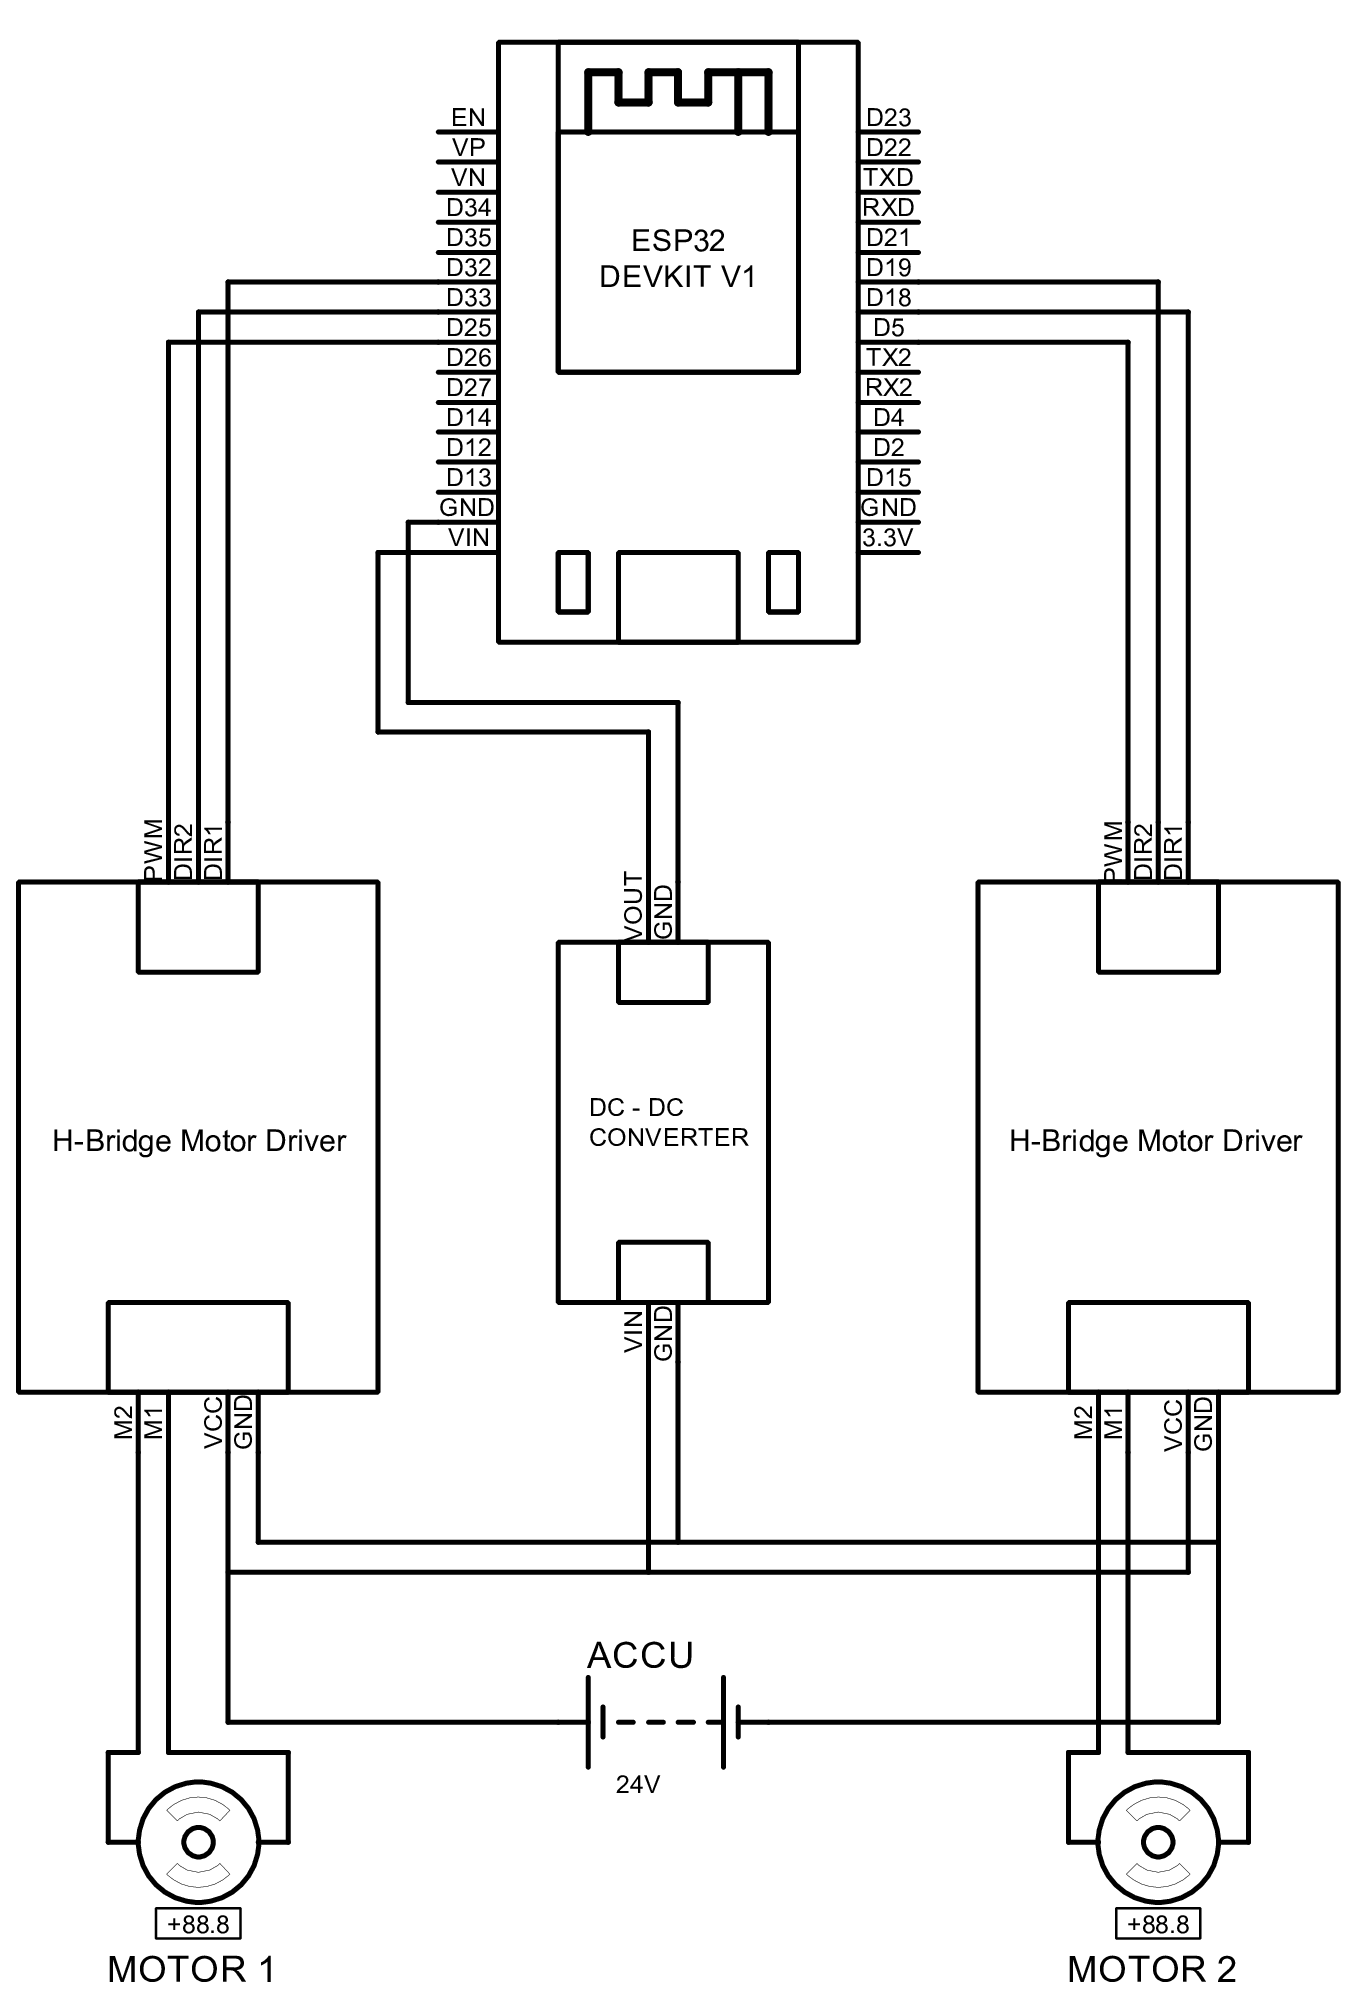
\includegraphics[scale=0.2]{gambar/Schematics.png}

  % Ubah dengan keterangan gambar yang diinginkan
  \caption{Skematik kontrol motor kursi roda}
  \label{fig:Skematik Kontrol motor Kursi roda.}
\end{figure}

\subsection{Perangkat Lunak}
\label{subsec:perangkatlunak}

Perangkat lunak yang digunakan dalam sistem ini terdiri dari beberapa modul, yang meliputi:

\begin{itemize}
    \item \textbf{Algoritma Deteksi YOLOv11}: YOLOv11 digunakan untuk mendeteksi manusia dalam gambar yang ditangkap oleh kamera. Model ini dilatih untuk mengenali bentuk dan posisi manusia sehingga kursi roda dapat mengikuti target dengan tepat.
    \item \textbf{Estimasi Pose MediaPipe}: MediaPipe digunakan untuk mendeteksi landmark tubuh manusia setelah objek terkunci. Framework ini dipilih karena kemampuannya dalam mendeteksi keypoints pada tubuh manusia dengan akurasi tinggi, bahkan dalam kondisi pencahayaan yang beragam.
    \item \textbf{Komunikasi Data}: Sistem menggunakan protokol MQTT untuk mengirimkan data antara ESP32 yang terhubung ke kamera dan unit kontrol utama.
    \item \textbf{Kontrol Motor}: Modul kontrol motor diimplementasikan pada ESP32 untuk mengatur arah dan kecepatan motor berdasarkan posisi target yang terdeteksi.
\end{itemize}

\subsubsection{Dataset Citra}
\label{subsubsec:datasetcitra}

Dataset citra yang digunakan dalam penelitian ini terdiri dari kumpulan gambar yang diambil menggunakan kamera OV5640. Objek yang dideteksi pada gambar ini adalah manusia, yang difungsikan sebagai target untuk diikuti oleh kursi roda. Dataset mencakup berbagai pose dan posisi manusia, serta kondisi pencahayaan yang berbeda, agar model YOLOv11 dapat dilatih secara optimal dalam mengenali target dalam berbagai situasi. Gambar-gambar ini diperoleh dari setiap frame video yang diambil menggunakan kamera yang terhubung dengan komputer. Proses pendeteksian dilakukan secara real-time untuk memastikan sistem mampu mengidentifikasi target secara berkelanjutan.

\subsubsection{Labeling}
\label{subsubsec:labeling}

Dataset citra yang telah diperoleh kemudian melalui proses labeling dan augmentasi menggunakan alat seperti Roboflow, yang menyediakan berbagai fitur untuk mempermudah proses ini. Proses labeling ini melibatkan impor dataset, pemberian label pada setiap gambar, dan augmentasi data. Labeling dilakukan untuk memastikan bahwa setiap objek dalam gambar dikenali dengan benar, terutama manusia yang menjadi target. Penamaan class harus konsisten dengan objek yang akan dideteksi untuk memastikan model YOLOv11 dapat dilatih dengan baik.

Selain itu, Roboflow juga menyediakan fitur preprocessing dataset yang membantu menstandarkan format gambar, misalnya mengubah ukuran semua gambar menjadi seragam. Langkah ini penting untuk menjaga konsistensi dataset sebelum melatih model. Beberapa fitur yang tersedia antara lain Auto-Orient, Resize, Grayscale, Auto Adjust Contrast, Isolate Objects, Static Crop, Tile, Modify Classes, dan Filter Null. Preprocessing ini memastikan bahwa data yang digunakan memiliki kualitas yang seragam untuk meningkatkan performa model.

Fitur augmentasi data juga disediakan untuk menambah variasi pada dataset. Augmentasi bertujuan untuk meningkatkan keragaman dalam dataset, yang pada akhirnya membantu meningkatkan performa model dalam mendeteksi manusia. Proses augmentasi ini sangat penting dalam tugas akhir ini karena membutuhkan variasi yang luas dalam data citra manusia, yang memungkinkan sistem lebih robust dalam berbagai kondisi.

\subsubsection{Klasifikasi YOLOv11}
\label{subsubsec:klasifikasiYOLOv11}

Dalam proses klasifikasi, setiap citra yang telah melalui proses labeling dikenali dengan menggunakan YOLOv11 yang telah dilatih untuk mendeteksi manusia pada citra. Model ini mampu mendeteksi keberadaan manusia secara akurat dan real-time, memungkinkan sistem untuk mengidentifikasi target dengan efisien. Setiap citra diproses oleh model YOLOv11, yang kemudian memberikan output berupa bounding box dan confidence score yang menunjukkan keberadaan manusia serta keyakinan model terhadap deteksi tersebut. Proses ini dilakukan secara real-time, memungkinkan sistem untuk memberikan umpan balik langsung ke kontrol kursi roda berdasarkan deteksi manusia dalam gambar.

Model YOLOv11 yang digunakan memiliki output kelas utama yaitu manusia. Model ini menghasilkan bounding box, yang menunjukkan area lokasi objek, dan confidence score untuk memberikan keyakinan deteksi. Algoritma YOLOv11 menggunakan Convolutional Neural Network (CNN) sebagai basisnya, yang berfungsi untuk mengekstraksi fitur dari gambar input, lalu memprediksi bounding box dan kelas objek langsung dari gambar tersebut. Proses ini diilustrasikan pada Gambar, yang menunjukkan blok diagram arsitektur model YOLOv11.

Lapisan deteksi pada YOLOv11 menghasilkan output yang mencakup bounding box dan confidence score untuk manusia yang terdeteksi, yang kemudian digunakan sebagai acuan dalam sistem untuk mengikuti target. Model ini dioptimalkan untuk dapat mengenali manusia dengan berbagai posisi dan kondisi pencahayaan, sehingga kursi roda dapat beradaptasi dengan pergerakan target dalam berbagai situasi secara efektif.

\subsubsection{Estimasi Pose MediaPipe}
\label{subsubsec:estimasi_pose_mediapipe}

Pada penelitian ini, pose manusia dideteksi menggunakan Python dengan library OpenCV dan MediaPipe. Proses dimulai setelah objek manusia terdeteksi dalam frame, di mana MediaPipe kemudian digunakan untuk mengidentifikasi landmark pada tubuh. MediaPipe dipilih karena kemampuannya mendeteksi titik kunci (keypoints) pada tubuh manusia dengan akurasi tinggi dalam berbagai kondisi pencahayaan dan posisi. Setelah landmark berhasil dideteksi, titik-titik yang relevan akan digambarkan menggunakan garis untuk membentuk kerangka sesuai dengan pose tubuh.

Proses deteksi diawali dengan inisialisasi kamera yang menangkap frame secara real-time. Setelah frame diterima, dilakukan pra-pengolahan seperti konversi gambar ke skala abu-abu untuk mengurangi kompleksitas dan meningkatkan kecepatan deteksi. Gambar yang telah dipra-pengolah tersebut kemudian diproses oleh model MediaPipe untuk mendeteksi pose.

Dalam penelitian ini, beberapa landmark yang dipilih untuk analisis adalah titik-titik pada siku, lengan bawah, dan bahu kanan serta kiri. Pemilihan titik-titik ini didasarkan pada visibilitas dan konsistensi dalam proses deteksi. Tabel menampilkan nomor dan nama keypoint yang digunakan dalam estimasi pose:

\begin{table}[H]
  \centering
  \caption{Tabel Keypoint yang digunakan}
  \label{tab:keypoints}
  \begin{tabular}{|c|c|}
    \hline
    Nomor Keypoint & Nama Keypoint \\
    \hline
    11 & RIGHT SHOULDER \\
    12 & LEFT SHOULDER \\
    14 & RIGHT ELBOW \\
    16 & RIGHT WRIST \\
    \hline
  \end{tabular}
\end{table}

Setelah landmark diperoleh, jarak antar titik pada piksel dihitung. Pengukuran ini dilakukan dengan menggunakan jarak Euclidean antara dua titik kunci, yang merupakan metode efisien untuk menghitung jarak dalam ruang dua dimensi. Nilai jarak ini kemudian digunakan sebagai acuan untuk pergerakan kursi roda mengikuti target di depan.

\subsubsection{Pemrosesan Citra}
\label{subsubsec:pemrosesan_citra}

Pemrosesan citra dilakukan untuk meningkatkan kualitas gambar yang diambil dari kamera dan mempermudah deteksi objek. Langkah-langkah pemrosesan citra meliputi konversi warna, penghilangan noise, dan pemfilteran tepi untuk menyorot bagian-bagian penting dari gambar.

\subsubsection*{Pembuatan Tracking ID untuk Mengunci Target}
\label{subsubsec:tracking_id}

Sistem ini memanfaatkan Ultralytics YOLO untuk mendeteksi target manusia dalam setiap frame, lalu memberikan ID unik pada setiap objek yang terdeteksi. ID tersebut berfungsi untuk mengidentifikasi dan melacak individu yang sama pada frame berikutnya, memungkinkan untuk terus mengikuti target meskipun terjadi pergerakan dalam frame. Deteksi yang akurat dan pemberian ID ini sangat penting agar kursi roda dapat merespons secara tepat terhadap perubahan posisi target.

\subsubsection*{Keputusan untuk Bergerak Maju}
\label{subsubsec:keputusan_bergerak_maju}

Setelah target terdeteksi dan tracking ID dibuat, sistem akan menghitung jarak antara kursi roda dengan target. Jika jarak target berada dalam kisaran yang aman dan berada di tengah frame, sistem akan mengirimkan perintah untuk bergerak maju. Hal ini dilakukan dengan menggunakan algoritma yang menghitung jarak dari bounding box target dan memastikan bahwa target berada pada posisi yang tepat untuk diikuti.

\subsubsection*{Keputusan untuk Berbelok ke Kiri}
\label{subsubsec:keputusan_belok_kiri}

Jika target bergerak ke arah kiri dan keluar dari batas tengah frame, kursi roda akan mengirimkan perintah untuk berbelok ke kiri. Sistem mendeteksi posisi target di bagian kiri frame dan memberikan instruksi ke motor untuk mengarahkan kursi roda ke kiri agar tetap dapat mengikuti pergerakan target secara optimal.

\subsubsection*{Keputusan untuk Berbelok ke Kanan}
\label{subsubsec:keputusan_belok_kanan}

Sebaliknya, jika target bergerak ke arah kanan dan keluar dari batas tengah frame, sistem akan mengirimkan perintah untuk berbelok ke kanan. Posisi target yang berada di sisi kanan frame akan memicu motor untuk berbelok ke kanan, memastikan kursi roda dapat menyesuaikan posisinya dengan target yang bergerak.

\subsubsection*{Keputusan Jika Target Menghilang dari Frame}
\label{subsubsec:keputusan_target_menghilang}

Apabila target menghilang dari frame, sistem akan mencari target berdasarkan posisi terakhir yang terdeteksi. Jika ada target baru yang terdeteksi di frame, sistem akan membuat tracking ID baru dan melanjutkan pelacakan terhadap target tersebut. Sistem akan menunggu hingga target muncul kembali dalam frame atau mendeteksi target baru untuk melanjutkan pelacakan. Pendekatan ini memastikan bahwa kursi roda bergerak sesuai arah terakhir ketika target tidak terlihat.

\subsubsection{Komunikasi Data}
\label{subsubsec:komunikasi_data}

Pada sistem ini, komunikasi data dilakukan menggunakan kombinasi WiFi dan ESP-NOW. WiFi digunakan untuk membangun Access Point pada ESP32 yang terhubung dengan kamera, memungkinkan streaming video real-time ke unit kontrol melalui jaringan lokal. Stream ini dapat diakses melalui server HTTP di port 81, di mana data video dari kamera diproses oleh unit kontrol untuk deteksi target.

Selain itu, ESP-NOW digunakan untuk pengiriman data secara langsung antara dua perangkat ESP32. Data yang diterima dari port 80 oleh ESP32 yang terhubung dengan kamera dikirimkan ke ESP32 lainnya (yang mengendalikan motor) melalui ESP-NOW. Protokol ini memungkinkan pertukaran data dengan latensi rendah tanpa memerlukan koneksi internet atau router eksternal. Dengan kombinasi ini, sistem dapat mempertahankan komunikasi yang cepat dan stabil, memastikan kursi roda dapat merespons pergerakan target secara real-time.

\subsubsection{Kontrol Motor}
\label{subsubsec:kontrol_motor}

Kontrol motor pada sistem kursi roda ini diimplementasikan menggunakan ESP32 yang bertindak sebagai pengendali utama untuk arah dan kecepatan motor. Setelah target manusia terdeteksi oleh kamera dan diproses oleh YOLOv11, informasi mengenai posisi target dikirim ke ESP32 untuk menentukan perintah pergerakan yang sesuai. Berdasarkan posisi target di dalam frame, ESP32 akan memberikan sinyal kepada driver motor untuk mengendalikan arah gerakan kursi roda, baik bergerak maju, berbelok ke kiri, berbelok ke kanan, atau berhenti.

Motor dikendalikan melalui sinyal PWM (Pulse Width Modulation) yang dihasilkan oleh ESP32, yang digunakan untuk mengatur kecepatan motor secara halus. Kombinasi sinyal arah dan PWM memungkinkan sistem untuk menggerakkan motor dengan responsif, baik untuk mengejar target, berbelok, atau berhenti secara tiba-tiba jika diperlukan. Selain itu, sistem juga menggunakan kontrol loop untuk terus memantau posisi target dan menyesuaikan pergerakan kursi roda secara real-time agar tetap dapat mengikuti target dengan akurat. Proses kontrol ini berlangsung terus-menerus untuk memastikan bahwa kursi roda selalu dapat beradaptasi dengan pergerakan target.

\subsubsection{Kode Program}
\label{subsubsec:kode_program}

Kode program yang digunakan dalam penelitian ini dimulai dengan inisialisasi variabel dan perangkat keras yang diperlukan, termasuk mengaktifkan kamera untuk menangkap gambar secara real-time. Setelah gambar diperoleh, algoritma YOLOv11 digunakan untuk mendeteksi keberadaan manusia dalam frame tersebut. Jika manusia terdeteksi, program melanjutkan dengan mengidentifikasi bounding box dan memberi label pada objek, yang kemudian digunakan untuk melacak objek tersebut di frame berikutnya. Setelah itu, framework MediaPipe diimplementasikan untuk mendeteksi landmark tubuh, seperti bahu, siku, dan pergelangan tangan, yang memungkinkan sistem memperoleh pose manusia secara lebih rinci.

\begin{figure}[H]
  \centering
  \resizebox{1\linewidth}{!}{
    \begin{tikzpicture}[node distance=2cm]
\node (start) [startstop] {Mulai};
\node (initVars) [process, below of=start] {Inisialisasi Variabel dan Hardware};
\node (captureFrame) [io, below of=initVars] {Ambil Frame dari Kamera};
\node (yoloDetect) [process, below of=captureFrame] {Deteksi Objek Menggunakan Yolo};
\node (A) [connector, below of=yoloDetect] {A};
\node (C0) [connector, left of=initVars, xshift=-1.5cm, yshift=-1cm] {C};

\node (A0) [connector, right of=start, xshift=4.5cm] {A};
\node (checkBoxes) [decision, below of=A0] {Deteksi Objek?};
\node (processBox) [process, below of=checkBoxes] {Proses Bounding Box};
\node (trackingID) [process, below of=processBox] {Proses Tracking ID};
\node (mediapipeProcessing) [process, below of=trackingID] {Deteksi Landmark Pose pada MediaPipe};
\node (B) [connector, below of=mediapipeProcessing, xshift=1.5cm] {B};

\node (B0) [connector, right of=A0, xshift=3.5cm] {B};
\node (calcDirection) [process, below of=B0] {Proses Kalkulasi Arah dan Jarak};
\node (controlWheelchair) [io, below of=calcDirection] {Kirim Data ke Kursi Roda};
\node (display) [io, below of=controlWheelchair] {Gambar Arah pada Frame};
\node (endLoop) [decision, below of=display, yshift=-.5cm] {Tombol 'q' Ditekan?};
\node (C) [connector, right of=endLoop, xshift=1cm, yshift=-1.5cm] {C};
\node (end) [startstop, below of=endLoop, yshift=-1cm] {Selesai};

\node (searchPerson) [process, below of=mediapipeProcessing, xshift=-3cm] {Memuat Arah dan Jarak Sebelumnya};

\draw [arrow] (start) -- (initVars);
\draw [arrow] (initVars) -- (captureFrame);
\draw [arrow] (captureFrame) -- (yoloDetect);
\draw [arrow] (yoloDetect) -- (A);
\draw [arrow] (C0) |- (captureFrame);

\draw [arrow] (A0) -- (checkBoxes);
\draw [arrow] (checkBoxes) -- node[anchor=west] {Ya} (processBox);
\draw [arrow] (processBox) -- (trackingID);
\draw [arrow] (trackingID) -- (mediapipeProcessing);
\draw [arrow] (mediapipeProcessing) -- +(0,-2cm);

\draw [arrow] (B0) -- (calcDirection);
\draw [arrow] (calcDirection) -- (controlWheelchair);
\draw [arrow] (controlWheelchair) -- (display);
\draw [arrow] (display) -- (endLoop);
\draw [arrow] (endLoop) -| node[anchor=south east] {Tidak} (C);
\draw [arrow] (endLoop) -- node[anchor=west] {Ya} (end);

\draw [arrow] (checkBoxes) -| node[anchor=south west] {Tidak} (searchPerson);
\draw [arrow] (searchPerson) -- (B);
\end{tikzpicture}
  }
  \caption{Flowchart program python}
\end{figure}

Program kemudian menghitung arah dan jarak target, yang digunakan untuk menentukan instruksi pergerakan kursi roda. Instruksi tersebut dikirimkan ke ESP32, yang mengendalikan motor kursi roda untuk mengikuti manusia secara otomatis. Selain itu, arah pergerakan digambarkan pada frame video yang ditampilkan sebagai bentuk visualisasi dari proses yang sedang berjalan. Program akan terus melakukan loop, menangkap gambar baru, memproses deteksi, dan mengirimkan perintah hingga pengguna menekan tombol 'q' untuk mengakhiri program.


\begin{figure}[H]
  \centering
  \resizebox{.7\linewidth}{!}{
    \begin{tikzpicture}[node distance=2cm]
\node (start) [startstop] {Mulai};
\node (getCurrentTime) [io, below of=start] {Ambil Waktu\\Saat ini};
\node (check_delay) [decision, below of=getCurrentTime, text width=2.5cm] {\emph{delay} \(\lor\) Data: C?};
\node (check_sent) [decision, below of=check_delay, yshift=-.5cm] {Sudah dikirim?};
\node (A) [connector, left of=check_sent, xshift=-1cm] {A};
\node (send_data) [process, below of=check_sent] {Mengirim data};
\node (sent_true) [process, below of=send_data] {Penanda data sudah dikirim};

\node (A0) [connector, right of=start, xshift=4cm, yshift=-.5cm] {A};
\node (check_update) [decision, below of=A0] {Data berubah?};
\node (send_C) [process, below of=check_update] {Mengirim 'C\textbackslash n'};
\node (check_input) [decision, below of=send_C] {Input: C?};
\node (update_data) [io, below of=check_input, text width=2.7cm] {Data diperbarui};
\node (sent_false) [process, below of=update_data] {Penanda data belum dikirim};
\node (stop) [startstop, below of=sent_false, xshift=-3cm] {Selesai};

\draw [arrow] (start) -- (getCurrentTime);
\draw [arrow] (getCurrentTime) -- (check_delay);
\draw [arrow] (check_delay) -- node[anchor=west] {Tidak} (check_sent);
\draw [arrow] (check_sent) -- node[anchor=west] {Tidak} (send_data);
\draw [arrow] (send_data) -- (sent_true);
\draw [arrow] (check_sent) -- node[anchor=north] {Ya} (A);

\draw [arrow] (A0) -- (check_update);
\draw [arrow] (check_update) -- node[anchor=west] {Ya} (send_C);
\draw [arrow] (send_C) -- (check_input);
\draw [arrow] (check_input) -- node[anchor=west] {Tidak} (update_data);
\draw [arrow] (update_data) -- (sent_false);

\draw [arrow] (check_delay) -| node[anchor=north east] {Ya} (stop);
\draw [arrow] (check_update) -| node[anchor=north west] {Tidak} (stop);
\draw [arrow] (check_input) -| node[anchor=north west] {Ya} (stop);
\draw [arrow] (sent_true) |- +(3cm,-1cm) -- (stop);
\draw [arrow] (sent_false) |- +(-3cm,-1cm) -- (stop);

\end{tikzpicture}
  }
  \caption{Flowchart regulasi arah}
\end{figure}

Regulasi arah kursi roda dilakukan melalui pengiriman data arah ke socket yang berhubungan dengan ESP32. Program mengecek apakah socket tersedia dan apakah data arah berubah, serta menetapkan penanda untuk menghindari pengiriman data yang berulang. Sebelum arah diubah, data 'C\textbackslash n' dikirim terlebih dahulu untuk memastikan kursi roda berhenti dan stabil sebelum menerima instruksi arah baru. Hal ini penting untuk mencegah gerakan yang tidak diinginkan atau perubahan arah yang terlalu mendadak. Setiap kali arah berubah setelah berhenti, data baru akan dikirim ke socket untuk mengontrol motor kursi roda.

Untuk ESP32 CAM, sistem dimulai dengan inisialisasi kamera yang terhubung ke ESP32. Langkah pertama adalah pengaturan kamera agar siap menangkap gambar lingkungan secara real-time. Kamera yang digunakan adalah OV5640 dengan resolusi 5MP, yang memungkinkan pengambilan gambar berkualitas tinggi untuk deteksi yang lebih akurat.

\begin{figure}[H]
  \centering
  \resizebox{.7\linewidth}{!}{
    \begin{tikzpicture}[node distance=2cm]

% Nodes
\node (start) [startstop] {Mulai};
\node (wifi) [process, below of=start] {Sambungkan ke Wi-Fi};
\node (wifiCheck) [decision, below of=wifi, text width=2cm] {Wi-Fi Terhubung?};
\node (mdns) [process, below of=wifiCheck] {Setup mDNS dan Port};
\node (A) [connector, below of=mdns] {A};

\node (A0) [connector, right of=start, xshift=4cm] {A};
\node (cameraInit) [process, below of=A0] {Inisialisasi Kamera};
\node (serverStart) [process, below of=cameraInit] {Mulai Server Kamera};
\node (ready) [io, below of=serverStart, text width=3.5cm] {Tampilkan URL\\untuk Akses Stream};
\node (end) [startstop, below of=ready] {Selesai};

% Arrows
\draw [arrow] (start) -- (wifi);
\draw [arrow] (wifi) -- (wifiCheck);
\draw [arrow] (wifiCheck) -- node[anchor=west] {Ya} (mdns);
\draw [arrow] (mdns) -- (A);
\draw [arrow] (A0) -- (cameraInit);
\draw [arrow] (cameraInit) -- (serverStart);
\draw [arrow] (serverStart) -- (ready);
\draw [arrow] (ready) -- (end);

\draw [arrow] (wifiCheck.west) -| node[anchor=north west] {Tidak} ++(-1,0) |- (wifi.west);
\end{tikzpicture}
  }
  \caption{Flowchart ESP-CAM}
\end{figure}

Sistem ini menerapkan protokol \emph{mDNS (Multicast DNS)} untuk secara otomatis memberikan nama unik pada setiap kamera. Setiap kamera terhubung dengan nama berbeda, seperti \emph{camera.local}, \emph{camera2.local}, dan seterusnya. Alokasi port untuk streaming diatur secara otomatis, misalnya melalui port \emph{81}, \emph{82}, dan seterusnya, dengan akses langsung ke \emph{endpoint} \emph{/stream}. Pendekatan ini memudahkan penambahan kamera tanpa perlu konfigurasi manual. Dengan proses pendaftaran otomatis, sistem dapat menyesuaikan diri untuk berbagai kebutuhan, seperti pemantauan dari berbagai sudut atau penggunaan kamera cadangan sebagai redundansi. Setiap perangkat diakses melalui jaringan lokal menggunakan URL unik, yang menyederhanakan manajemen dan akses kamera dalam jaringan.

Selain itu, penggunaan server WiFi memungkinkan unit kontrol (seperti komputer atau laptop) mengakses data gambar secara langsung melalui jaringan lokal. Hal ini sangat berguna untuk menganalisis gambar secara lebih rinci dan mengambil keputusan kontrol yang lebih kompleks, seperti perubahan arah atau kecepatan kursi roda berdasarkan posisi target dalam frame. Dengan demikian, proses ini memberikan fleksibilitas yang tinggi dalam mengatur pergerakan kursi roda berdasarkan data yang diperoleh dari kamera.

Dengan memastikan koneksi Wi-Fi sebelum mengaktifkan kamera pada ESP32-CAM, konsumsi daya dapat dikelola secara optimal, sehingga panas yang dihasilkan tidak berlebih. Hal ini menjaga suhu modul kamera dan chip ESP32 dalam batas yang aman, yang berperan penting dalam mencegah overheating. Pengendalian suhu yang baik juga mendukung fungsi sensor kamera dan komponen elektronik lainnya, sehingga perangkat dapat beroperasi dengan kinerja maksimal dalam jangka panjang.

Frame yang ditangkap oleh kamera dikirim melalui alamat lokal tertentu yang juga digunakan dalam kode program Python untuk melakukan streaming data. Data arah yang diterima dari client kemudian diteruskan ke ESP32 B melalui TCP/IP dengan unit kontrol untuk mengontrol kursi roda. Sistem ini dirancang untuk memastikan komunikasi yang cepat dan handal, sehingga kursi roda dapat merespons pergerakan target dengan tepat.

\begin{figure}[H]
  \centering
  \resizebox{1\linewidth}{!}{
    \begin{tikzpicture}[node distance=2cm]
% Nodes
\node (start) [startstop] {Mulai};
\node (init) [process, below of=start] {Inisialisasi Arduino, WiFi, PWM dan Pin};
\node (connect) [process, below of=init] {Menyambungkan Serial WiFi dan Server};
\node (setup) [process, below of=connect] {Setup PinMode, ledc-Setup, ledcAttachPin};
\node (A) [connector, below of=setup, xshift=3cm, yshift=-.5cm] {A};

\node (A0) [connector, right of=start, xshift=4cm] {A};
\node (connected?) [decision, below of=A0, text width=2cm] {Perangkat Terhubung?};
\node (msg?) [decision, below of=connected?, yshift=-.5cm] {Pesan Diterima?};

\node (stop) [startstop, right of=connected?, xshift=3cm] {Stop};
\node (readstr) [process, right of=msg?, xshift=3cm] {Read String sampai terdapat '\textbackslash n'};
\node (extract) [process, below of=readstr] {Ekstrak String menjadi Arah dan Kecepatan};
\node (move) [io, below of=msg?, text width=3.5cm] {Menggerakkan Motor Kursi Roda};

% Arrows
\draw [arrow] (start) -- (init);
\draw [arrow] (init) -- (connect);
\draw [arrow] (connect) -- (setup);
\draw [arrow] (setup) |- ++(0,-1.55cm) -| (A);

\draw [arrow] (A0) -- (connected?);
\draw [arrow] (connected?) -- node[anchor=east] {Ya} (msg?);
\draw [arrow] (connected?) -- node[anchor=south] {Tidak} (stop);
\draw [arrow] (msg?) -- node[anchor=south] {Ya} (readstr);
\draw [arrow] (msg?.west) -| node[anchor=north west] {Tidak} (A);
\draw [arrow] (readstr) -- (extract);
\draw [arrow] (extract) -- (move);
\draw [arrow] (move.south) |- ++(0,-.5) -| (A);
\end{tikzpicture}
  }
  \caption{Flowchart ESP Motor}
\end{figure}

Pada sisi ESP32 Motor, perangkat dimulai dengan inisialisasi berbagai komponen, seperti PWM, WiFi, dan pin untuk mengendalikan motor. Setelah terhubung ke WiFi, ESP32 B menunggu pesan dari server yang berfungsi sebagai pusat kendali. Jika pesan diterima, string yang mengandung informasi arah dan kecepatan akan diekstrak, kemudian diolah untuk menentukan pergerakan motor kursi roda. Sistem menggunakan data ini untuk mengatur arah dan kecepatan motor, yang memastikan kursi roda dapat mengikuti target secara akurat dan responsif. Proses ini dilakukan secara berulang untuk setiap update data yang diterima, memungkinkan kursi roda menyesuaikan gerakan dengan perubahan posisi target secara real-time.

% Ubah judul dan label berikut sesuai dengan yang diinginkan.
\section{Hasil dan Pembahasan}
\label{sec:hasildanpembahasan}

Pada penelitian ini dipaparkan skenario pengujian yang dilakukan, termasuk kondisi lingkungan pengujian, perangkat keras dan perangkat lunak yang digunakan, serta parameter-parameter yang diuji. Informasi detail mengenai konfigurasi dan prosedur pengujian disajikan agar hasil pengujian dapat direplikasi dengan konsisten.

\subsection{Hasil Pengujian Performa Menggunakan Confusion Matrix}
\label{subsec:hasilperformaconfisionMatrix}

Bagian ini membahas hasil pengujian performa deteksi objek menggunakan Confusion Matrix. Nilai seperti True Positive, True Negative, False Positive, dan False Negative dianalisis untuk menilai akurasi dan efektivitas deteksi.

\subsection{Pengujian Berdasarkan FPS}
\label{subsec:pengujianberdasarkanfps}

Pengujian ini dilakukan untuk menganalisis kecepatan pemrosesan sistem dalam satuan Frame per Second (FPS). FPS yang tinggi menunjukkan bahwa sistem dapat bekerja dengan baik secara real-time. Grafik hasil pengujian disertakan untuk memudahkan visualisasi performa.

\subsection{Pengujian Berdasarkan Response Time}
\label{subsec:pengujianberdasarkanresponsetime}

Bagian ini mengukur waktu yang dibutuhkan sistem untuk merespons setiap perubahan lingkungan atau perintah yang diterima. Response Time sangat penting untuk mengukur responsivitas sistem dalam skenario dinamis.

\subsection{Performa Keberhasilan Tracking}
\label{subsec:performakeberhasiltracking}

Bagian ini mengevaluasi keberhasilan sistem dalam melakukan tracking terhadap objek target. Tingkat keberhasilan dianalisis untuk mengetahui keandalan sistem dalam berbagai skenario.

\subsection{Pengujian Kesesuaian Jarak Deteksi}
\label{subsec:pengujiankesesuaianjarakdeteksi}

Pengujian dilakukan untuk mengukur kemampuan sistem dalam mendeteksi objek pada berbagai jarak  dan menganalisis performa sistem pada jarak-jarak tersebut.

\subsection{Performa Pergerakan Mengikuti Objek}
\label{subsec:performaakurasiobjek}

Analisis dilakukan untuk mengukur seberapa akurat sistem dapat mengikuti objek target, termasuk mempertahankan jarak yang tepat dan tidak kehilangan objek dalam berbagai kondisi.

\subsubsection{Saat berada didalam frame}
\label{subsubsec:dalamframe}

Bagian ini membahas kemampuan sistem dalam mengikuti objek saat berada didalam tangkapan layar. Tantangan yang dihadapi dan solusi yang diterapkan diuraikan.

\subsubsection{Saat berada diluar frame}
\label{subsubsec:luarframe}

Bagian ini membahas kemampuan sistem dalam mengikuti objek saat berada diluar frame. Tantangan yang dihadapi dan solusi yang diterapkan diuraikan.

\subsubsection{Belok kiri saat berada didalam frame}
\label{subsubsec:belokkiri}

Bagian ini membahas kemampuan sistem dalam mengikuti objek saat berbelok ke kiri, mirip dengan bagian sebelumnya.

\subsubsection{Belok Kanan saat berada didalam frame}
\label{subsubsec:belokkanan}

Bagian ini membahas kemampuan sistem dalam mengikuti objek saat berbelok ke kanan, mirip dengan bagian sebelumnya.

\subsection{Performa Keberhasilan Mengikuti}
\label{subsec:performamengikuti}

Bagian ini menguji apakah sistem dapat mengikuti objek pada lajur khusus, seperti jalur sempit atau berbelok yang membutuhkan manuver khusus.

\subsection{Pembahasan Hasil}
\label{subsec:pembahasanhasil}

Bagian ini membahas hasil-hasil pengujian secara keseluruhan dan memberikan insight mengenai performa sistem.

\subsubsection{Performa Deteksi Objek}
\label{subsec:performadeteksiobjek}

Bagian ini menjelaskan kekuatan dan kelemahan deteksi objek yang ditemukan selama pengujian.

\subsubsection{Kecepatan Pemrosesan (FPS)}
\label{subsec:kecepatanpemrosesan}

Menganalisis kecepatan pemrosesan secara keseluruhan dan pengaruhnya terhadap performa sistem real-time.

\subsubsection{Response Time}
\label{subsec:responsetime}

Membahas hasil pengujian response time dan faktor-faktor yang mempengaruhi waktu respons.

\subsubsection{Performa Keberhasilan Tracking}
\label{subsec:performatracking}

Membahas tingkat keberhasilan sistem dalam melacak objek dan kondisi yang mempengaruhi performa.

\subsubsection{Kesesuaian Jarak Deteksi}
\label{subsec:kesesuaianjarak}

Diskusi tentang performa sistem dalam mendeteksi objek pada berbagai jarak yang telah diuji.

\subsubsection{Performa Pergerakan Mengikuti Objek}
\label{subsec:akurasiikutiobjek}

Evaluasi akurasi dalam mengikuti objek target, termasuk kondisi yang dapat menyebabkan kegagalan.

\subsubsection{Performa Keberhasilan Mengikuti}
\label{subsec:keberhasilanmengikuti}

Menguraikan keberhasilan sistem dalam mengikuti objek saat menghadapi belokan dan lajur khusus.
% Ubah judul dan label berikut sesuai dengan yang diinginkan.
\section{Kesimpulan}
\label{sec:kesimpulan}

% Ubah paragraf-paragraf pada bagian ini sesuai dengan yang diinginkan.

Berdasarkan hasil pengujian yang telah dilakukan, dapat diambil kesimpulan sebagai berikut:

\begin{enumerate}
  \item Model dengan Metrics tertinggi yang telah di-training dengan berbagai konfigurasi adalah model dengan skor mAP di IoU 0.5 tertinggi sebesar 81.85\%. Adapun nilai yang didapatkan ini sudah cukup baik untuk melakukan penghindaran dilihat pada hasil performa penghindaran yang sangat baik.
  \item Performa NUC dalam pengujian FPS menghasilkan Nilai yang lebih rendah ketimbang Laptop pribadi Penulis dengan selisih 7.029 fps.
  \item Rata - rata delay yang didapatkan pada pengujian adalah sekitar 0.2494 detik dan rata- rata nilai inference yang didapatkan 139.4899 ms atau 0.1394 detik.
  \item Hasil menunjukkan bahwa deteksi menggunakan \emph{Bounding box} dan Landmark bahu lebih akurat pada jarak yang lebih jauh (150 cm dan 100cm), sedangkan landmark lengan lebih akurat pada jarak yang lebih dekat (50 cm). Dimana rata-rata \emph{difference} terbaik bounding box yaitu pada jarak 150cm sebesar 3.2 cm, rata-rata \emph{difference} landmark bahu terbaik yaitu pada jarak 100cm sebesar 2.2 cm dan rata-rata \emph{difference} landmark lengan terbaik yaitu pada jarak 50cm sebesar 1.93 cm.
  \item Hasil Performa Deteksi menunjukan hasil yang memuaskan dalam 30 sampel pengujian. Dengan presentasi keberhasilan sebesar 100\% yang menunjukan bahwa sistem yang dibuat dapat menghindari manusia dengan sangat baik.

\end{enumerate}

\section{Saran}
\label{chap:saran}

Untuk pengembangan lebih lanjut pada penelitian selanjutnya, adapun saran yang bisa diberikan antara lain:

\begin{enumerate}

  \item Variasi dataset yang lebih ditingkat untuk meningkatkan performa deteksi
  \item Menggunakan Device yang memiliki performa yang lebih baik untuk fps yang lebih tinggi
  \item Meningkatkan performa grid deteksi dengan melakukan penyesuaian yang lebih detail untuk pemetaan yang lebih baik lagi.
  \item Menggunakan pendingin device saat melakukan pengujian di ruangan terbuka agar tidak mengalami penurunan performa.
\end{enumerate}
% Ucapan terima kasih jika ada
% \section{Ucapan Terima Kasih}
% \label{sec:ucapanterimakasih}

% Penulis mengucapkan terima kasih kepada Kementerian Riset, Teknologi, dan Pendidikan Tinggi Republik Indonesia atas \lipsum[1]

% Menampilkan daftar pustaka dengan format IEEE
\bibliographystyle{IEEEtran}
\bibliography{pustaka/pustaka.bib}

% Menyeimbangkan bagian akhir di kedua kolom
\balance

\end{document}